% !TeX encoding = UTF-8
% !TeX program = xelatex
% !TeX spellcheck = en_US

\documentclass[degree=master]{thuthesis}
  % 学位 degree:
  %   doctor | master | bachelor | postdoc
  % 学位类型 degree-type:
  %   academic(默认)| professional
  

\usepackage[ruled,vlined]{algorithm2e}


% 论文基本配置,加载宏包等全局配置
% !TeX root = ./thuthesis-example.tex
% Settings for basic information of thesis
% 论文基本信息配置
\newcommand{\junz}[1]{{\color{red}{\bf\sf [zj: #1]}}}

\thusetup{
  %******************************
  % 注意:
  %   1. 配置里面不要出现空行
  %   2. 不需要的配置信息可以删除
  %   3. 建议先阅读文档中所有关于选项的说明
  %******************************
  %
  % 输出格式
  %   选择打印版(print)或用于提交的电子版(electronic),前者会插入空白页以便直接双面打印
  %
  output = print,
  degree=master,
  language=english,
  % 标题
  %   可使用“\\”命令手动控制换行
  %
  % Input your title in CHINESE & English: 
  title  = {深度强化学习的对抗鲁棒性评测 \\
  \textbf{Evaluating the Adversarial Robustness of Deep Reinforcement Learning}},
  % Input your title* in ENGLISH
  title* = {Evaluating the Adversarial Robustness of Deep Reinforcement Learning},
  %
  % 学位
  %   1. 学术型
  %      - 中文
  %        需注明所属的学科门类,例如:
  %        哲学、经济学、法学、教育学、文学、历史学、理学、工学、农学、医学、
  %        军事学、管理学、艺术学
  %      - 英文
  %        博士:Doctor of Philosophy
  %        硕士:
  %          哲学、文学、历史学、法学、教育学、艺术学门类,公共管理学科
  %          填写“Master of Arts“,其它填写“Master of Science”
  %   2. 专业型
  %      直接填写专业学位的名称,例如:
  %      教育博士、工程硕士等
  %      Doctor of Education, Master of Engineering
  %   3. 本科生不需要填写
  %
  % Please do no change:
  degree-name  = {工学硕士},
  degree-name* = {Master of Science},
  %
  % 培养单位
  %   填写所属院系的全名
  %
  department = {计算机科学与技术系},
  %
  % 学科
  %   1. 学术型学位
  %      获得一级学科授权的学科填写一级学科名称,其他填写二级学科名称
  %   2. 工程硕士
  %      工程领域名称
  %   3. 其他专业型学位
  %      不填写此项
  %   4. 本科生填写专业名称,第二学位论文需标注“(第二学位)”
  %
  % discipline  = {计算机科学与技术},
  discipline* = {Computer Science and Technology},
  %
  % 姓名
  %
  % Please input your full name in CHINESE
  author  = {刘大为},
  % Please input your full name in ENGLISH
  author* = {Davide Liu},
  %
  % 指导教师
  %   中文姓名和职称之间以英文逗号“,”分开,下同
  %
  % Please input your supervisor's full name in Chinese, then comma, followed by 教授 (for Professor) and 副教授 (for Associate Prof.)
  supervisor  = {朱军, 教授},
  % Please input your supervisor's title (ie Professor) and followed by full name in English
  supervisor* = {Professor Zhu Jun},
  %
  % 副指导教师
  %
  % associate-supervisor  = {陈文光, 教授},
  % associate-supervisor* = {Professor Chen Wenguang},
  %
  % 联合指导教师
  %
  % joint-supervisor  = {某某某, 教授},
  % joint-supervisor* = {Professor Mou Moumou},
  %
  % 日期
  %   使用 ISO 格式;默认为当前时间
  %
  % Please change the date as required
  date = {2021-05-05},
  %
  % 是否在中文封面后的空白页生成书脊(默认 false)
  %
  include-spine = false,
  %
  % 密级和年限
  %   秘密, 机密, 绝密
  %
  % secret-level = {秘密},
  % secret-year  = {10},
  %
  % 博士后专有部分
  %
  % clc                = {分类号},
  % udc                = {UDC},
  % id                 = {编号},
  % discipline-level-1 = {计算机科学与技术},  % 流动站(一级学科)名称
  % discipline-level-2 = {系统结构},          % 专业(二级学科)名称
  % start-date         = {2011-07-01},        % 研究工作起始时间
}

% 载入所需的宏包

% 可以使用 nomencl 生成符号和缩略语说明
% \usepackage{nomencl}
% \makenomenclature

% 表格加脚注
\usepackage{threeparttable}

% 表格中支持跨行
\usepackage{multirow}

% 固定宽度的表格。放在 hyperref 之前的话,tabularx 里的 footnote 显示不出来。
% \usepackage{tabularx}

% 跨页表格
% \usepackage{longtable}

% 量和单位
\usepackage{siunitx}

% 定理类环境宏包
\usepackage{amsthm}
% 也可以使用 ntheorem
% \usepackage[amsmath,thmmarks,hyperref]{ntheorem}

% 参考文献使用 BibTeX + natbib 宏包
% 顺序编码制
\usepackage[sort]{natbib}
\bibliographystyle{thuthesis-numeric}

% 著者-出版年制
% \usepackage{natbib}
% \bibliographystyle{thuthesis-author-year}

% 本科生参考文献的著录格式
% \usepackage[sort]{natbib}
% \bibliographystyle{thuthesis-bachelor}

% 参考文献使用 BibLaTeX 宏包
% \usepackage[backend=biber,style=thuthesis-numeric]{biblatex}
% \usepackage[backend=biber,style=thuthesis-author-year]{biblatex}
% \usepackage[backend=biber,style=apa]{biblatex}
% \usepackage[backend=biber,style=mla-new]{biblatex}
% 声明 BibLaTeX 的数据库
% \addbibresource{ref/refs.bib}

% 定义所有的图片文件在 figures 子目录下
\graphicspath{{figures/}}

% 数学命令
\newcommand\dif{\mathop{}\!\mathrm{d}}  % 微分符号

% hyperref 宏包在最后调用
\usepackage{hyperref}



\begin{document}

% 封面
\maketitle

% 学位论文指导小组、公开评阅人和答辩委员会名单
% List of committee on your defense session
% !TeX root = ../thuthesis-example.tex

\begin{committee}[name={THESIS REVIEWERS AND DEFENSE COMMITTEE}]

  %%\newcolumntype{C}[1]{@{}>{\center\arraybackslash}p{#1}}
  \newcolumntype{C}[1]{@{}>{\arraybackslash}p{#1}}

  %\section*{指导小组名单}

  %\begin{center}
  %  \begin{tabular}{C{3cm}C{3cm}C{9cm}@{}}
  %    李XX & 教授     & 清华大学 \\
  %    王XX & 副教授   & 清华大学 \\
  %    张XX & 助理教授 & 清华大学 \\
  %  \end{tabular}
  %\end{center}

  % Reviewer's names
  \begin{center}
    \section*{公开评阅人名单}
  \end{center}

  \begin{center}
    \begin{tabular}{C{3cm}C{3cm}C{9cm}@{}}
      黄民列 & 副教授   & 清华大学                    \\
      胡晓林 & 副教授 & 清华大学                    \\
    \end{tabular}
  \end{center}

  % Defense committee
  \begin{center}
      \section*{答辩委员会名单}
  \end{center}
  

  \begin{center}
    \begin{tabular}{C{2.75cm}C{2.98cm}C{4.63cm}C{4.63cm}@{}}
      主席 &  周立柱                & 教授                    & 清华大学       \\
      委员 & 朱军               & 教授                    & 清华大学   \\
      & 邓志东               & 教授                    & 清华大学       \\
          & 汪东升                 & 教授                    & 清华大学       \\
       &  黄民列 & 副教授   & 清华大学                    \\
      秘书 & 戴音                  & 讲师              & 清华大学       \\
    \end{tabular}
  \end{center}

\end{committee}



% 也可以导入 Word 版转的 PDF 文件
% \begin{committee}[file=figures/committee.pdf]
% \end{committee}


% 使用授权的说明
% Copyright page
\copyrightpage
% 将签字扫描后授权文件 scan-copyright.pdf 替换原始页面
% Please replace this page with a SCANNED version with your signature
% \copyrightpage[file=scan-copyright.pdf]

\frontmatter
% !TeX root = ../thuthesis-example.tex

% 中英文摘要和关键字
% Abstract in CHINESE
% Requirements: 800-1000 CHINESE characters, it should not exceed 1 page maximum. You are allowed a maximum of 5 keywords in total
\begin{abstract}
现有文献已经广泛研究了针对深度学习模型的对抗攻击,并提出了几种防御方法来保护神经网络免受恶意对抗样本的攻击。然而,大多数工作主要集中在处理图像数据(例如,图像分类任务)的卷积神经网络上。近年来,由于卷积神经网络具有从原始像素提取重要图像特征的能力,这些模型还广泛应用于深度强化学习算法中。这些算法只需向模型提供像素观察值并据此预测特定的动作,即可从头开始学习策略。尽管如此,该领域的大多数研究都针对提升智能体性能,即最大程度地提高它们获得的收益。现有针对智能体鲁棒性的研究中,较少关注一类将其引向危险状态的对抗性攻击,这类攻击将减少智能体所获得的收益。本文首先研究了一些最常见的深度强化学习算法的鲁棒性。其次,分析了上述算法面对设计恶意策略的攻击的脆弱性。第三,研究了它们在策略和算法之间的可转移性。最后,研究了在防御机制存在的情况下,基于图像的攻击制定有效的对抗性观察的能力。本文提出,除针对策略攻击外,还应该针对图像攻击方法来评估策略的鲁棒性,因为某些图像攻击与特定的策略攻击结合可以更好地发挥作用。本文提出采用与受害方策略相同算法训练的替代策略进行的对抗性观察具有更好的可传递性,而且使用与替代策略算法相似的算法来训练替代策略时,可传递性更为有效。

  % 关键词用“英文逗号”分隔,输出时会自动处理为正确的分隔符
  % Input your keywords in CHINESE, separated by a "english comma" to ensure correct formatting. 
  \thusetup{
    keywords = {强化学习, 对抗决策, 对抗攻击, 鲁棒性},
  }
\end{abstract}

% Corresponding abstract in English
% Note that the keywords and the contents of the abstract should match with the CHINESE version
\begin{abstract*}
  Adversarial attacks against deep learning models have been widely studied in literature, and several defense methods have then been proposed to protect neural networks against malicious adversarial examples. However, most of the work is mainly focused on convolutional neural networks dealing with image data such as for image classification tasks. In recent years, thanks to their ability to extract important image features from raw pixels, those models have also found wide application in deep reinforcement learning algorithms which are able to learn a policy from scratch simply by feeding them with pixel observations and predict specific actions accordingly. Still, most of the research in this field is addressed on improving agents' performance in terms of maximizing their earned reward, while relatively little has been done to study their robustness against adversarial attacks that are able to mislead those policies toward dangerous states, thus reducing the obtained reward. In this thesis work, we first investigated the robustness of some of the most common deep reinforcement learning algorithms. Second, we showed their vulnerability against attacks that design malicious policies. Third, we studied their transferability propriety across policies and algorithms. Finally, we investigated the ability of image-based attacks to craft effective adversarial observations, even in presence of defense mechanisms. We hypothesize that policy robustness should be evaluated not only against policy attacks but also against image attack methods since some image attacks work better in combination with particular policy attacks. Moreover, we showed that adversarial observations crafted on surrogate policies trained with the same algorithm of the victim policy benefit of a better transferability, and we also empirically demonstrated that transferability is more effective when the surrogate policy is trained with an algorithm similar to the algorithm used to train the victim policy.


  % Use comma as seperator when inputting
  \thusetup{
    keywords* = {Reinforcement learning, Adversarial policies, Adversarial attacks, Robustness},
  }
\end{abstract*}


% 目录
% Contents
\tableofcontents

% 插图和附表清单
% List of figures and tables
\listoffiguresandtables  % 插图和附表清单
% \listoffigures           % 插图清单
% \listoftables            % 附表清单

% 符号对照表
% Denotions and abbreviations
% !TeX root = ../thuthesis-example.tex

% Please put your abbreviations, denotations, nomenclatures in here.
\begin{denotation}[3cm]
  \item[DRL] Deep Reinforcement Learning
  \item[DQN] Deep Q-Network
  \item[MDP] Markov Decision Process
  \item[A2C] Advantage-Actor-Critic
  \item[PPO] Proximal policy optimization
  \item[SGD] Stochastic Gradient Descent
  \item[\(\theta\)] Weights of a Neural Network
  \item[\(\pi\)] Reinforcement Learning Policy
  \item[FGSM] Fast Gradient Sign Method
  \item[MI-FGSM] Momentum Iterative-Fast Gradient Sign Method
  \item[PGD] Projected Gradient Descent
\end{denotation}



% 也可以使用 nomencl 宏包,需要在导言区
% \usepackage{nomencl}
% \makenomenclature

% 在这里输出符号说明
% \printnomenclature[3cm]

% 在正文中的任意为都可以标题
% \nomenclature{PI}{聚酰亚胺}
% \nomenclature{MPI}{聚酰亚胺模型化合物,N-苯基邻苯酰亚胺}
% \nomenclature{PBI}{聚苯并咪唑}
% \nomenclature{MPBI}{聚苯并咪唑模型化合物,N-苯基苯并咪唑}
% \nomenclature{PY}{聚吡咙}
% \nomenclature{PMDA-BDA}{均苯四酸二酐与联苯四胺合成的聚吡咙薄膜}
% \nomenclature{MPY}{聚吡咙模型化合物}
% \nomenclature{As-PPT}{聚苯基不对称三嗪}
% \nomenclature{MAsPPT}{聚苯基不对称三嗪单模型化合物,3,5,6-三苯基-1,2,4-三嗪}
% \nomenclature{DMAsPPT}{聚苯基不对称三嗪双模型化合物(水解实验模型化合物)}
% \nomenclature{S-PPT}{聚苯基对称三嗪}
% \nomenclature{MSPPT}{聚苯基对称三嗪模型化合物,2,4,6-三苯基-1,3,5-三嗪}
% \nomenclature{PPQ}{聚苯基喹噁啉}
% \nomenclature{MPPQ}{聚苯基喹噁啉模型化合物,3,4-二苯基苯并二嗪}
% \nomenclature{HMPI}{聚酰亚胺模型化合物的质子化产物}
% \nomenclature{HMPY}{聚吡咙模型化合物的质子化产物}
% \nomenclature{HMPBI}{聚苯并咪唑模型化合物的质子化产物}
% \nomenclature{HMAsPPT}{聚苯基不对称三嗪模型化合物的质子化产物}
% \nomenclature{HMSPPT}{聚苯基对称三嗪模型化合物的质子化产物}
% \nomenclature{HMPPQ}{聚苯基喹噁啉模型化合物的质子化产物}
% \nomenclature{PDT}{热分解温度}
% \nomenclature{HPLC}{高效液相色谱 (High Performance Liquid Chromatography)}
% \nomenclature{HPCE}{高效毛细管电泳色谱 (High Performance Capillary lectrophoresis)}
% \nomenclature{LC-MS}{液相色谱-质谱联用 (Liquid chromatography-Mass Spectrum)}
% \nomenclature{TIC}{总离子浓度 (Total Ion Content)}
% \nomenclature{\textit{ab initio}}{基于第一原理的量子化学计算方法,常称从头算法}
% \nomenclature{DFT}{密度泛函理论 (Density Functional Theory)}
% \nomenclature{$E_a$}{化学反应的活化能 (Activation Energy)}
% \nomenclature{ZPE}{零点振动能 (Zero Vibration Energy)}
% \nomenclature{PES}{势能面 (Potential Energy Surface)}
% \nomenclature{TS}{过渡态 (Transition State)}
% \nomenclature{TST}{过渡态理论 (Transition State Theory)}
% \nomenclature{$\increment G^\neq$}{活化自由能(Activation Free Energy)}
% \nomenclature{$\kappa$}{传输系数 (Transmission Coefficient)}
% \nomenclature{IRC}{内禀反应坐标 (Intrinsic Reaction Coordinates)}
% \nomenclature{$\nu_i$}{虚频 (Imaginary Frequency)}
% \nomenclature{ONIOM}{分层算法 (Our own N-layered Integrated molecular Orbital and molecular Mechanics)}
% \nomenclature{SCF}{自洽场 (Self-Consistent Field)}
% \nomenclature{SCRF}{自洽反应场 (Self-Consistent Reaction Field)}



% 正文部分
% Main thesis
\mainmatter
% !TeX root = ../thuthesis-example.tex

% Your chapter title here
% Please make sure that the title is in CAPITALS
% All section and subsection headings, use capital letters where required
\chapter{INTRODUCTION}
\label{introduction}

This chapter gives a brief introduction about the major breakthroughs of the field of deep reinforcement learning starting from a simple DQN \cite{mnih2013playing} to more advanced algorithms such as AlphaZero \cite{silver2017mastering} and AlphaStar \cite{Arulkumaran_2019}. It gives an idea of the complexity of the environments and the challenges these AIs have to overcome and explains why training robust policies is so important for most applications in the real world.    

\section{Major breakthroughs of deep reinforcement learning}
With the advent of deep learning, neural networks have quickly invaded the field of reinforcement learning giving birth to a new branch called deep reinforcement learning (DRL). First steps were taken back in 2013 when \cite{mnih2013playing} used a Deep Q-Network (DQN) to learn to play a number of classic Atari games only by observing their environment from raw pixels using a simple convolutional network. Starting from zero knowledge, the agent explores strategical policies by itself, and after training for a sufficient number of frames, it hopefully learns to play on the target environment, sometimes even achieving super-human performance. Later on, the DRL field had another important breakthrough in 2016, when a famous AI developed by DeepMind known as AlphaGo \cite{alphago} defeated for the first time in the history a 9-dan Go player, Lee Sedol, for 4 games to 1 playing against him without handicaps. The strategy game of GO was, at the time, considered very hard to be solved by AI algorithms due to its enormous number of possible states (about \(10^{170}\)) an agent has to deal with. One year later, its evolution, AlphaZero \cite{silver2017mastering}, even managed to defeat Ke Jie who at the time of the match was ranked first among all human players worldwide. One year later, in 2019, a more general version of AlphaZero, MuZero \cite{Schrittwieser_2020}, successfully mastered the game of Chess, Go, and Shogi without knowing the rules of the games and is even able to generalize to single-agent environments such as Atari games without changing its architecture. In 2018, a new agent developed by Uber, Go-Explore \cite{ecoffet2019goexplore}, for the first time solved the game Montezuma’s Revenge with a score of over 43,000 points, which is almost 4 times the previous state of the art. Montezuma’s Revenge is well known for being a very hard environment for RL agents since its rewards are very sparse, and many tasks have to be done before getting any score. One year later, in 2019, another agent developed by DeepMind, AlphaStar \cite{Arulkumaran_2019}, managed to beat a top-10 player of Starcraft for 5 to 0 as well as defeating 86\% of medium level players. Finally, also in 2019, Tencent MOBA-playing AI system \cite{ye2019mastering} beat 99.81\% of professional human opponents in full 1v1 games of the MOBA \textit{Honor of Kings}. The actor-critic agent included several novel strategies such as control dependency decoupling, action mask, target attention, and dualclip PPO. Master the game of \textit{Honor of Kings} is far more challenging than Go since in a normal match could be encountered about \(10^{600}\) possible states.

\section{Importance of training robust policies}
However, besides performance, safety also plays a fundamental role when deploying DRL-based models in real-world applications. An agent that achieves super-human skills in a certain task but that fails to complete its goal when its inputs are subjected to minimal perturbations can't be considered as a reliable system. Even worse, this lack of robustness may even lead to dangerous situations. In a scenario where an agent driving an autonomous car is fed with adversarial examples, it may be deceived by the environment to choose to take sub-optimal actions, thus degrading its performance. In an even more dangerous scenario, an attacker may craft a sequence of adversarial samples so to lead the agent toward a dangerous target state, thus causing a possible collision or committing an infringement. Besides self-driving cars and videogames, DRL finds application in other critical systems such as training robots used in manufacturing, enhancing the performance of electric power systems, and evaluating trading strategies in the financial sector. Given the critical issues of the above-mentioned scenarios, it is reasonable to think that robustness plays a critical role and these systems should be prevented from being fooled by adversarial observations crafted by a malicious agent.  Hence, the direction of this thesis project concerns studying the effects of adversarial attacks and defenses on deep reinforcement learning algorithms so to evaluate their robustness under different levels of adversary knowledge and their possible defenses, so to make these systems more reliable and usable in the real world.

\section{Thesis overview}
The work in this thesis thus investigates the robustness of some of the most common deep reinforcement learning algorithms and shows their vulnerability both against malicious policies with the goal to mislead the agent toward sub-optimal states and against adversarial attacks aimed at crafting more effective adversarial observations. Malicious or adversarial policies are generated employing policy adversarial attacks which will be introduced in chapter \ref{sec:rla}. Since the evaluated policies take images as input, policy adversarial attacks, in turn, perform image attacks on input observations so to change the victim policy's actions distribution toward an adversarial one. For this reason, we believe that, in order to do a comprehensive study on policies robustness, merely evaluating policy attacks is not enough since these attacks are conditioned by the performance of the image attacks they rely on. Image adversarial attacks will be introduced in chapter \ref{sec:ima}.

However, before going on with the main body of this thesis, it is important to have a clear concept of what is a {\it policy}, an {\it algorithm}, and what we mean for {\it transferability} in our context. A {\it policy} is a model that outputs a probability distribution over actions and it is trained using a reinforcement learning {\it algorithm}. However, two policies trained with the same algorithm may not necessarily be the same policy since a change in the random seed used to train the network implementing each policy would result in its weights having different parameters. Note that two policies trained or equipped with different defense mechanisms are also different policies since the defense method would influence their behavior. Furthermore, we have {\it policy transferability} when adversarial perturbations for the target policy are generated using another policy trained with the same algorithm and for the same task. Similarly, in the case of {\it algorithm transferability}, adversarial perturbations for the target policy are generated using another policy trained with a different algorithm for the same task. This is the same concept of attack transferability on image classification models but applied to the reinforcement learning domain. Moreover, when in the following chapters we are going to refer to a policy trained with algorithm \(A\) on environment \(E\) we are simply going to call it \(E-A\). For instance, Pong-DQN corresponds to a policy trained with DQN on the environment of Pong.

Overall, the main contributions of this work are the following:
\begin{itemize}
    \item \textbf{Study policy attacks transferability over policies and algorithms}: We computed the {\it reward vs attack frequency} curves of different policy attacks under a fixed threat model so to measure their effectiveness and their transferability against policies and algorithms \cite{huang2017adversarial}. We repeated the experiment for a total of 3 algorithms, 5 policy attacks, and 2 environments.
    \item \textbf{Study policy attacks transferability against defended policies}: We computed the {\it reward vs attack frequency} curves of different policy attacks under a fixed threat model so to measure their effectiveness and their transferability against defended policies and defended algorithms. We repeated the experiment for a total of 3 algorithms, 2 policy attacks, and 2 environments.
    \item \textbf{Benchmark of the robustness of defended policies against white-box image attacks methods}: We compared the curves of victim policies' average reward and success rate of different white-box attack methods attacking input observations under a fixed threat model and over increasing values of perturbations' strength \(\epsilon\). Victim policies have also been protected with different defense methods so as to have a better idea of the effectiveness of each attack and the robustness of these defended policies. These curves, introduced in \cite{dong2019benchmarking}, are also known as robustness curves and are used as major evaluation metrics to measure image classification models' robustness.
\end{itemize}

The present thesis work is structured in the following way. Chapter \ref{sec:drl} reviews the policies trained to conduct the experiments and the evaluated environments, chapter \ref{sec:ima} introduces the concept of adversarial attacks and defenses on images and explains some common white-box attacks used as backbone to implement policies adversarial attacks and defenses. Chapter \ref{sec:rla} gives a general overview of adversarial attacks on policies as well as possible defense methods. Chapters \ref{sec:exp1}, \ref{sec:exp2} and \ref{sec:exp3} show, analyze and discuss the results obtained in each of the three experiments respectively. Finally, \ref{sec:conclusions} gives a general discussion and conclusion about the work that has been carried out and points out some future research directions.
      
% !TeX root = ../thuthesis-example.tex

% Input your chapter title here
\chapter{DEEP REINFORCEMENT LEARNING}
\label{sec:drl}

This chapter first gives a brief overview of the theory behind reinforcement learning and then introduces the three deep learning algorithms used during the experiments carried out in this thesis work, namely DQN \cite{mnih2013playing}, A2C \cite{mnih2016asynchronous} and PPO \cite{schulman2017proximal}.

\section{Deep reinforcement learning}
Deep reinforcement learning (DRL) usually involves one or more agents interacting with an environment following a policy \(\pi\), like in a Markov Decision Process (MDP), where their goal is to improve their policy such to maximize their earned reward. More specifically, during training, the agent is provided with an observation \(s_t\) of the environment for each timestep \(t=0,1,2,...\), and it has to respond with an action \(a_{t}\). Afterwards, the environment provides a reward \(r(a_t,s_t)\), the next state \(s_{t+1}\), and a discount factor \(\gamma_t\). As regards to the selection of actions, they are selected according to a policy \(\pi\), modeled by a neural network with weights \(\theta\) that defines a probability distribution over the actions for each state. So, starting from state \(s_t\) encountered at time \textit{t}, we can define the discounted cumulative reward \(R_t\) as
\begin{equation}
R_t=\sum_{i=0}^{\infty}\gamma^{i}r_{t+i+1}.
\end{equation}
Thus, considering an episode starting at time \(t=0\) and terminating at time \(T\), the expected discounted reward of a policy \(\pi\) is defined as
\begin{equation}
R_0=\sum_{i=0}^{T-1}\mathbb{E}_{a_i\sim \pi(s_i)}[\gamma^i r(a_i,s_i)].
\end{equation}
Following, we are going to review in more details the three algorithms that have been employed to conduct this thesis work.


\section{Deep Q-Network}
Deep Q-network (DQN) \cite{mnih2013playing} is a neural network used to implement the Q-learning algorithm. More specifically, it learns an estimate of the Q-value \(Q(s,a,\theta)\) parameterized by the parameters \(\theta\) of the network (online network). The Q-value, which measures the value of choosing a particular action when in a particular state, can be defined according to the following recursive formula:
\begin{equation} \label{equation:Qvalue}
Q_{\theta_t}(s_{t},a_{t})=r_{t}+\gamma Q_{\theta_{t}} ((s_{t+1},a_{t+1})|s_{t},a_{t},\theta_{t}).
\end{equation}
Its architecture is composed of a first convolutional neural network (CNN) that takes as input a state \(s_t\) and learns to detect increasingly abstract features from it. Subsequently, a dense classifier maps the high-level extracted features to an output layer with one neuron per action in order to approximate the corresponding action value. The parameters of the network are trained by gradient descent to minimize the following loss function:
\begin{equation} \label{equation:DQN}
L_t(\theta_t)=(r_{t+1}+\gamma_{t+1}\max_{a'}Q_{\theta^{-}}(s_{t+1},a')-Q_{\theta_t}(s_t,a_t))^2.
\end{equation}
During training, a batch of experiences is randomly picked from the replay memory which is a sort of dataset storing the agent’s past experiences defined as the tuple \((s_t, a_t, r(a_t,s_t), s_{t+1})\). The experience replay technique prevents the network from learning from strongly correlated experiences that break the i.i.d. assumption of many popular stochastic gradient-based algorithms, as well as avoiding the rapid forgetting of possibly rare experiences that would be useful later on. Because of the experience replay, DQN is an off-policy algorithm since some sampled experiences might be explored with an older version of the online policy. The gradient of the loss is then back-propagated only into the parameters \(\theta\) of the online network which is used to select actions. The term \(\theta^-\) represents the parameters of a target network, a periodic copy of the online network which is not directly optimized and is used to estimate the maximum expected reward in equation (\ref{equation:DQN}). During training, the parameters of the online network are periodically copied into the ones of the target network so to update its weights. The advantage introduced by having an independent target network is to make the target Q-value independent with respect to the predicted Q-value when computing the loss so as to increase training stability. Overall, the Q-value calculated by the target network has more accuracy since it has access to at least the first reward term to calculate it. In order to encourage exploration, in particular during the early stage of training, greedy actions are taken with probability 1-\(\epsilon\) otherwise are performed random actions so to discover new policies that may lead to higher rewards.

\section{Advantage actor-critic}
Advantage Actor-Critic (A2C) \cite{mnih2016asynchronous} is formed by a neural network parameterized by \(\theta\) with 2 output layers: the first one is a softmax layer with weights \(\theta_\pi\) and outputs a policy \(\pi(a_t|s_t; \theta_\pi)\) (actor), the second one consists of a linear output for the value function \(V(s_t; \theta_v)\) (critic) parameterized by \(\theta_v\). Both the policy and the value function are periodically updated by gradient descent computing the gradient as
\begin{equation} \label{equation:A2C}
\nabla_\theta=\log \pi(a_t|s_t;\theta_\pi)A(a_t,s_t;\theta_v),
\end{equation}
\begin{equation} \label{equation:advantage}
A(a_t,s_t;\theta_v)=R_t-V(s_t;\theta_v),
\end{equation}
where \(A(a_t,s_t;\theta_v)\) is an estimate of the advantage function which measures the relative importance of each action respect to the state \(s_t\). The formula to compute the gradient derives from the loss function which is simply the negative log likelihood of the predicted action multiplied by the advantage. It also exists an asynchronous version called A3C which relies on several asynchronous agents, each of them interacting with its own copy of the environment, that accumulate gradients and periodically send them to the global network to perform updates. Agents running in parallel, possibly using different exploration policies, are likely to explore different parts of the environment, thus increasing samples' diversity and decreasing their correlation. Other benefits brought by using asynchronous agents consist of a linear reduction of training time based on the number of parallel agents, and the absence of an experience replay. This method is on-policy since it sequentially learns over its observed states. Note that Actor-Critic doesn't have an explicit hyper-parameter to regulate its grade of exploration since it trains a stochastic policy where exploration is done by sampling actions according to the actions probabilities defined by the actor network. Over the course of training, the policy will learn to become progressively less random.

\section{Proximal Policy Optimization}
Proximal Policy Optimization (PPO) \cite{schulman2017proximal} is a model-free on-policy algorithm that aims to balance among ease of implementation, sample complexity, and ease of tuning. PPO tries to compute an update at each step that minimizes the cost function while ensuring that the deviation from the previous policy is relatively small:
\begin{equation} \label{equation:PPO}
L^{CLIP}(\theta)=\mathbb{E}_t[\min(\frac{\pi_\theta(a_t|s_t)}{\pi_{\theta_{old}}(a_t|s_t)}A_t,clip(\frac{\pi_\theta(a_t|s_t)}{\pi_{\theta_{old}}(a_t|s_t)},1-\epsilon,1+\epsilon)A_t)],
\end{equation}
where the clipping operator prevents the maximization of the objective to lead to an excessively large policy update by constraining it in the interval \([1-\epsilon,1+\epsilon]\) and \(A_t\) is the advantage function computed as in equation (\ref{equation:advantage}). The architecture of the network involved in this algorithm is similar to A2C giving as output a distribution over actions and a value function used to compute the value of the advantage. Both functions are periodically updated after collecting a certain amount of trajectories. Moreover, PPO can run \(N\) parallel actors to collect the data, and then sample mini-batches of \(T\) timesteps to optimize the loss for \(K\) epochs using SGD.
% !TeX root = ../thuthesis-example.tex

% Input your chapter title here
\chapter{ADVERSARIAL ATTACKS ON IMAGES}
\label{sec:ima}

Since the policy attacks included in this thesis work by perturbing the image observations given in input to the victim policies, this chapter reviews some of the most common image attacks, their threat model and introduces some common defense methods to counter them.

\section{Adversarial attacks on images}
Since the advent of deep convolutional networks used for image classification \cite{NIPS2012_4824}, the computer vision field has been subjected to many important breakthroughs with the aim to further improve the classification accuracy obtained on many images classification tasks \cite{he2015deep} \cite{zhang2020resnest}. However, despite their high accuracy, those models lack robustness since they can be easily deceived by adversarial examples \cite{goodfellow2014explaining}. More formally, an adversarial example is a \textit{sample input data that has been modified very slightly in a way that is intended to cause a machine learning classifier to misclassify it} \cite{kurakin2016adversarial}. In fact, to be effective, an adversarial example should be misclassified by deep learning models, but not by the human brain. Therefore, only small changes can be made to the original input image \textit{x} (legitimate example) to craft the adversarial example \(x_{adv}\)=\textit{x}+\(\delta\), where \(\delta\) is also known as adversarial noise. The distance introduced by the noise between \textit{x} and \(x_{adv}\) is usually defined by the \(l_{p}\) norm of the difference between the original and the adversarial sample for some p=0,..,\(\infty\). Hence, an adversarial example \(x_{adv}\) has to satisfy the constraint \(||x_{adv}-x||_p\leq \epsilon\) (adversarial constraint), where smaller \(\epsilon\) values correspond to smaller input perturbations, thus leading to less perceptible changes under the condition that \(x_{adv}\) is misclassified. Moreover, images adversarial attacks can be designed to achieve two different goals:
\begin{itemize}
    \item \textbf{Untargeted}: Untargeted attacks aim at making the model predict any class different from the correct one without targeting at any desired class. Formally speaking, given a classifier \textit{f} and the true label \textit{y}, an adversarial example would cause \(f(x_{adv})\neq y\). Hence, untargeted attacks' goal consists of maximizing the loss of the attacked model respect to the true label \(y\), namely, \(\max \: L(x_{adv}, y)\), under the assumption \(||x_{adv}-x||_p\leq \epsilon\). Given the relaxed constraints the adversarial examples are subjected to, these kinds of attacks are usually easier to perform.
    \item \textbf{Targeted}: Conversely, targeted attacks try to mislead the model's prediction toward a specific class \textit{y'}, that is, \(f(x_{adv})=y'\), where \(y'\neq y\). The loss function can then be formulated as \(\min L(x_{adv}, y')\) always under adversarial constraints. In this way, given the input \(x_{adv}\), it will be more likely that the attacked model would predict the target class \(y'\) rather than any other class. More sophisticated policy attacks usually require crafting adversarial observation in a targeted way so to force the victim agent to perform some required actions.
\end{itemize}
For example, if we want an agent simply to have its performance degraded, attacking under untargeted settings would be enough since preventing it to take the best action would naturally lower its total earned reward. However, if our goal is to control the agent by making it choose some predefined actions such as to lead it to a particular state, then adversarial attacks should be performed under targeted settings. Finally, adversarial attacks are also divided into two main categories depending on how much information is available regarding the model under attack:
\begin{itemize}
    \item \textbf{White-box attacks}: Under this setting, the adversary has full access and knowledge of the model, that is, the architecture of the model, its parameters, gradients, and loss respect to the input as well as possible defense mechanisms are known to the attacker \cite{goodfellow2014explaining}. Thus, it is not particularly difficult to attack models under this condition, and common methods exploit model's output gradients to generate adversarial examples. Only attacks belonging to this category have been evaluated in this work.
    \item \textbf{Black-box attacks}: In this category of attacks, the adversary has zero or very little knowledge about the model. Thus existing methods often rely on training a similar model or an ensemble of them. These methods work because, generally, adversarial examples that fool one model are likely to fool another similar model. Furthermore, in practice, this is the most likely kind of attack, since, in normal circumstances, attackers don't have the possibility to access much of the models' knowledge. Other methods exploit knowledge about the accuracy of the prediction or only the label to craft adversarial examples \cite{wiel2017decisionbased}.
\end{itemize}
Both white and black-box attacks are possible when attacking DRL algorithms and it depends on how much knowledge is known regarding the network defining the policy of the agents. Conversely, adversarial defenses aim to protect deep learning models from adversarial attacks, namely, making models more robust against adversarial examples. In this context, research on adversarial robustness resembles a minimax game where attackers constantly try to exploit more powerful techniques to fool deep learning models while, at the same time, defenders have to invent new defense methods to guard against these malicious attacks.

\subsection{Generating adversarial examples}
In the next sections, have been reported some of the most common white-box attacks on images that are often also used to attack DRL agents. Moreover, these methods can also be used to attack images under black-box settings by crafting adversarial examples attacking similar models and then exploiting the transferability propriety of the adversarial examples to fool the target model \cite{dong2017boosting} or they can be directly applied to perform black-box attacks after estimating gradients by querying the target model \cite{Chen_2017}.

\subsection{FGSM}
Fast Gradient Sign Method (FGSM) \cite{goodfellow2014explaining} is a basic one-step gradient-based approach that is able to find an adversarial example in a single step by maximizing the loss function \( L(x_{adv}, y)\) with respect to the input \(x\) and then adding back the sign of the output gradients to \(x\) so to produce the adversarial example \(x_{adv}\)
\begin{equation}
x_{adv}=x+\epsilon \cdot sign(\nabla_x L(x, y)),
\end{equation}
where \(\nabla_x L(x, y)\) is the gradient of the loss respect to the input \(x\), and the equation is expected to meet the \(l_{\infty}\) norm bound by design. This method works because adding a perturbation to the legitimate input such to maximize its loss respect to the correct label \textit{y} decreases the likelihood that \textit{y} could be predicted given the input \(x_{adv}\). Mathematically, it moves the adversarial example in one direction toward the border between the true class and some other class \cite{dong2017boosting}. This method is sometimes implemented without the {\it sign} operator (FGM) and it yields similar results to the version with sign \cite{agarwal2018explainable}.

\subsection{I-FGSM}
Basic iterative methods \cite{kurakin2016adversarial} iteratively apply FGSM with a small step size \(\alpha\). Thus, the iterative version of FGSM (I-FGSM) can be expressed as
\begin{equation}
x_{adv}^{t+1}=x_{adv}^{t}+\epsilon \cdot \alpha \cdot sign(\nabla_x L(x_{adv}^{t}, y)),
\end{equation}
where \(x_{adv}^{0}=x\) is the legitimate example. There are several ways to make the adversarial example satisfy the norm bound. For example, \(x_{adv}\) could be clipped into the \(\epsilon\) vicinity of x or set \(\alpha=\epsilon/T\) with \(T\) being the number of iterations. \cite{kurakin2016adversarial} proved that iterative methods exploit much finer perturbations which do not destroy the image even with higher \(\epsilon\) and at the same time confuse the classifier with a higher rate. Their drawback is that iterative methods are a little bit slower than their one-step counterparts.
%, and more importantly, they show poor performance on transferability, which is a fundamental propriety in black-box attacks.

\subsection{MI-FGSM}
Momentum iterative gradient-based methods \cite{dong2017boosting} integrate momentum into iterative fast gradient method to generate adversarial examples satisfying the \(l_{p}\) norm bound. Traditionally, momentum is a technique for accelerating gradient descent algorithms by accumulating a velocity vector in the gradient direction of the loss function across iterations. However, this concept can also be applied to generate adversarial examples and obtain tremendous benefits. As it was for the learning rate update, the first step consists of updating the momentum \(g_t\) by accumulating the velocity vector in the gradient direction as 
\begin{equation}
g_{t+1}=\mu \cdot g_{t} + \frac{\nabla_x L(f(x, y)}{||\nabla_x L(x, y)||_p},
\end{equation}
where \(\mu\) is a decay factor. Next, the adversarial example \(x_{adv}^{t}\) is perturbed in the direction of the sign of \(g_{t}\) with a step size \(\alpha\) as
\begin{equation}
x_{adv}^{t+1}=x_{adv}^{t}+\alpha \cdot sign(g_{t+1}).
\end{equation}
In each iteration, the current gradient \(\nabla_x L(x, y)\) is normalized by the \(l_{p}\) distance of itself because the authors noticed that the scale of the gradients in different iterations varies in magnitude.

\subsection{PGD}
Projected gradient descent (PGD) \cite{madry2019deep} is another iterative algorithm that exploits projected gradient descend to iteratively craft adversarial examples as:
\begin{equation}
x_{adv}^{t+1}=\pi_{x+S}(x_{adv}^{t} +\alpha \cdot sign(\nabla_x L(x_{adv}^{t}, y))),
\end{equation}
where S is the set of all the allowed perturbations. Projected gradient descent performs one step of standard gradient descent, and then clips all the coordinates to be within the \(l_p\) ball. Moreover, in order to explore a large part of the loss landscape, the algorithm is restarted from many points within the \(l_p\) ball around data points taken from the evaluation set. Thanks to this large number of observations, the authors realized that all the local maxima found by PGD have similar loss values, both for normally trained networks and for adversarially trained networks, thus pointing out that robustness against the PGD adversary yields robustness against all first-order adversaries such as SGD based attacks. This conclusion also leads to the fact that as long as the adversary only uses gradients of the loss function with respect to the input, it will not find significantly better local maxima than PGD.

\subsection{C\&W}
The method proposed by Carlini \& Wagner \cite{carlini2016evaluating} relies on the initial formulation of adversarial example and formally defines the problem of finding an adversarial instance for an image \textit{x} as a minimization problem of a continuous function:
\begin{equation} \label{eq:CW}
\min \: ||\delta||_p+c \cdot L(x+\delta, y),
\end{equation}
under the condition that \((x+\delta)\in [0,1]^n\). The function \(f\) is an objective function such that \(L(x+\delta, y)\neq y\) if and only if \(L(x+\delta, y)<=0\). Finally, the term \textit{c} is a suitable chosen hyper-parameter. Moreover, to ensure that the modification yields a valid image, the adversarial noise \(\delta\) is constrained such that \(0\leq x_i+\delta_i\leq 1 \: \forall i\) (here assuming image pixels to be in the range [0,1]). One way to do it, is to replace \((x+\delta)\) with \((1+\tanh(w))/2\) so that the optimization problem in (\ref{eq:CW}) becomes an unconstrained minimization problem in \textit{w}.

\section{Defending against adversarial examples}
Extensive research in developing effective defense mechanisms in order to build robust models and safeguard them against adversarial attacks has also been conducted. One very promising technique is robust training which aims to make a classifier robust against small internal perturbations. Some possible strategies are based on adversarial training by adding generated adversarial examples to the training data \cite{goodfellow2014explaining}, defensive distillation which consists of retraining a network using previously generated soft-labels \cite{papernot2016distillation}, or another technique consists of training robust models with regularization such to train the defended model to ignore small perturbations \cite{hein2017formal}. Another category of defense methods that we are going to examine consists of input transformation. This method is not applied during training but only during inference by transforming the inputs right before feeding them to the classifier with the aim to make adversarial perturbations less effective.

\subsection{Adversarial training}
Adversarial training (AT) is a very simple and intuitive defense method to protect a model against adversarial examples. The first step consists of generating adversarial examples using different attack methods on the target model. In the second step, these adversarial examples are merged to the original training set so to form an augmented training set and finally the target model is retrained on the augmented training set. When adversarial examples are crafted with PGD we have PGD-adversarial training which can train very robust deep networks but it is much more expensive than traditional training due to the iterative design of PGD. In contrast, FGSM-adversarial training is typically faster but less effective \cite{wong2020fast}.

\subsubsection{JPEG compression}
JPEG compression \cite{dziugaite2016study} is a simple input transformation method that converts each input image to JPEG before it is fed to the target network. It has been studied that compressing an image can partially remove possible adversarial perturbations and, at the same time, elude the human perception that no transformation has been applied. However, in practice, this method is not very effective since it degrades the performance of the model while not cleaning completely an image from all the adversarial perturbations. To remedy this problem, \cite{das2018shield} proposes to vaccinate a policy by retraining it on JPEG compressed images multiple times on multiple compression qualities, and use an ensemble of these models to get the final classification label.

\subsubsection{Feature squeezing}
Feature squeezing \cite{Xu_2018} is another input transformation method that reduces the search space available to an adversary by compressing different features vectors in the original space into a single sample. Digital computers usually represent images as an array of pixels each of them representing a specific color (RGB images) or a shadow of grey (greyscale images). Thus, reducing bit depth can reduce the space that an adversarial has to craft perturbations possibly limiting the drop in accuracy that this compression may lead to. For example, an 8-bit greyscale image provides \(2^8=256\) values for each pixel which if reduced to 5-bits we would have only \(2^5=32\) values for each pixel that could be changed to create an adversarial example.
% !TeX root = ../thuthesis-example.tex

% Input your chapter title here
\chapter{ADVERSARIAL ATTACKS ON POLICIES}
\label{sec:rla}

This chapter explains in detail the policy attacks adopted in the experiments and defines their threat model. It gives an overview of both single and multi-agent attacks as well as possible defense methods.

\section{Adversarial attacks on policies}
As for adversarial attacks in other domains such as image or graph data, we can always define the properties of threat models, that is, a set of assumptions about the adversary’s goals, knowledge, and, in the reinforcement learning case, also the number of controllable agents interacting in the same environment. These conditions are specified by threat models so to determine under which conditions a defense is designed to be effective. Firstly, we can classify adversarial attacks on policies into two different categories based on the goal they are designed to achieve \cite{lin2017tactics}:
\begin{itemize}
    \item \textbf{Untargeted}: In the case of untargeted attacks, the goal is to decrease the performance of the victim agent, namely, causing it to take sub-optimal actions with respect to its learned policy so to reduce its total earned reward.
    \item \textbf{Targeted}: Targeted attacks aim to control the agent by making it take a sequence of some predefined actions so to lure it to a particular state. This kind of attack is more difficult to achieve since causing the agent to take a malicious specific action and leading it to a specific state are two tasks whose solutions are not immediate.
\end{itemize}
Secondly, depending on the knowledge the attacker has about the model defining the agent's policy and the algorithm used, we can individuate other three categories of attacks \cite{s2017adversarial}:
\begin{itemize}
    \item \textbf{White-box}: full knowledge about environment, training algorithm, and network.
    \item \textbf{Black-box I: Algorithm is known but not the policy}: the adversary has access to the training environment and knowledge of the training algorithm and hyperparameters. It also knows the neural network architecture of the target policy network, but not its random initialization. 
    \item \textbf{Black-box II: Both algorithm and policy are not known}: under these settings, the adversary has no knowledge of the training algorithm or hyperparameters, but it only knows the environment. Hence, it may need to craft its attacks using a different algorithm. In practice, it is often the case that an adversary does not have complete access to the neural network of the target policy \cite{huang2017adversarial}.
\end{itemize}
Thirdly, we have another important distinction based on whether other controllable agents can interact in the same environment or not \cite{gleave2020adversarial}: 
\begin{itemize}
    \item \textbf{Single-agent}: In the environment is present only one agent that is not directly controllable, thus it can be only deceived by adding adversarial noise to the input observations it receives.
    \item \textbf{Multi-agent}: In the same environment of the victim agent are also present other agents that can be controlled and trained to assume a particular behavior that could modify the environment such as to create observations that may deceive the victim.
\end{itemize}
In the next sections, we are first going to discuss the single-agent scenario and then we will briefly focus on the multi-agent one. All the reviewed attacks are summarized in table \ref{table:1}.

\begin{table}
  \centering
  \caption{General overview of the attacks methods reviewed in this thesis and their corresponding categories.}
  \begin{tabular}{ccc}
    \toprule
    Attack method & Goal & Scenario               \\
    \midrule
    Uniform Attack & Untargeted & Single-agent \\ 
    Strategically-Timed Attack & Untargeted & Single-agent \\
    Enchanting Attack & Targeted & Single-agent \\
    Critical Point Attack & Untargeted & Single-agent\\
    Critical Strategy Attack & Untargeted & Single-agent\\
    Adversarial Policy & Untargeted & Single-agent/Multi-agent\\
    \bottomrule
  \end{tabular}
  \label{table:1}
\end{table}

\subsection{Single-agent adversarial attacks}
In the case of single-agent DRL scenarios, the only way the attacker has to fool the victim agent consists of adding small perturbations to the observations it receives as input. In fact, one of the most interesting features that made DRL agents so popular is that they are only fed with some observations of the environment in order to learn or exploit their policy. Commonly, these observations only consist of raw or pre-processed images composed of pixels, thus vulnerable to adversarial attacks targeting images.

Following, we are going to introduce some of the most significant adversarial attacks under single-agent scenario. When it is required to make the victim agent choosing or avoiding a particular action, it can be used any method for adversarial attacks on images to craft adversarial observations, and sometimes, this procedure will be omitted without loss of generality.

\subsection{Uniform attack}
The first attack proposed to degrade the performance of DRL agents is the Uniform Attack \cite{s2017adversarial}, it falls into the family of untargeted attacks and consists of slightly perturbing all images the agent observes so to cause it choosing sub-optimal actions. Perturbations can be crafted with any existing method to attack image classification models under untargeted settings. This simple attack can be regarded as a direct extension of the adversarial attack on a CNN-based classification system since the adversarial example at each time step is computed independently of the adversarial examples at other time steps. However, it shows good results both in terms of transferability against algorithms and policies, in particular for large values of perturbations \(\epsilon\). However, despite being particularly effective against DQN, it doesn't scale well against more robust algorithms such as A2C and PPO.

\subsection{Strategically-timed attack}
Instead of attacking at every time step in an episode, Strategically-Timed attack \cite{lin2017tactics} selects a subset of time steps to attack the agent. Given the difficulty of the problem, the authors decided to subdivide it into two separate tasks: \textit{when to attack} and \textit{how to attack}. To solve the first task, it can be defined a function \(c\) that computes the preference of the agent in taking the most preferred action over the least preferred action at the current state \(s_t\). Hence, the \(c\) function can be defined as 
\begin{equation}
c(s_t)=max_{a_t}\pi(s_t,a_t)-min_{a_t}\pi(s_t,a_t).
\end{equation}
Then, the adversary attacks the victim agent at time step \(t\) when the relative action preference function \(c\) has a value greater than a threshold parameter \(\beta\). The intuition behind this is that when an agent strongly prefers a specific action, it means that it is critical to perform that action, otherwise the accumulated reward will be reduced. To solve the second task, it can be used any image adversarial attack method to change the preferred action of the agent from the originally most preferred one to the originally least preferred one. Finally, the authors of this attack found that, on average, the strategically-timed attack can reach the same effect of the uniform attack \cite{s2017adversarial} by attacking 25\% of the time steps in an episode. 

\subsection{Enchanting attack}
The goal of the Enchanting attack \cite{lin2017tactics} is to lead the DRL agent from current state \(s_t\) to a specified target state \(s_g\) after \(H\) steps. Also this attack is divided into two tasks: the first one consists of planning a sequence of actions for reaching the target state \(s_g\) from the current state \(s_t\). In the second one, it is crafted an adversarial example to lure the victim to take the first action of the planned action sequence using any image adversarial attack method. In particular, the first task is accomplished by training a video prediction model to predict a future state given a sequence of actions using a generative model. Since the goal of the enchanting attack is to reach the target state \(s_g\), the success of the attack is based on the distance between \(s_g\) and \(s_{t+H}\) predicted by the model. Regarding the action selection, are computed a sequence of actions using a sampling-based cross-entropy method, and is selected the sequence leading to a final state \(s_{t+H}\) which is the closest to \(s_g\). Based on evaluations on some Atari games, this method reaches an accuracy of about 70\% with a drop of performance on environments with a high level of stochasticity.

\subsection{Critical point attack}
In Critical Point Attack \cite{sun2020stealthy} the adversary builds a domain-specific model to predict the states of the next few steps, as well as the damage consequences of all possible attack strategies. As for many other attacks, also this method is performed in many stages. Firstly, the adversary uses observations of the target environment to train a prediction model \(P\) such that it takes a state-action pair as input and outputs a deterministic prediction of the next state. Then, it defines different strategies as sequences of \(N\) actions starting at step \(t\). In the third step, the adversary assesses the potential damage of all possible strategies from state \(t\) to \(t+M\) with \(M>=N\) and the last \(M-N\) steps following the normal policy. Next, the adversary calculates the value of the last state \(T(s_{t+M})\) using the function \(T\) which is a domain-specific divergence function defined as the least favorable state to reach. After computing \(T(s'_{t+M})\) for each attack strategy and the normal policy, the Danger Awareness Metric (DAM) between the two states, one reached because of a malicious policy and the other one following the normal policy is defined as
\begin{equation}
DAM=|T(s'_{t+M})-T(s_{t+M})|.
\end{equation}
If DAM is larger than a threshold \(\delta\), the adversary will conduct the attacks in the next \(N\) steps following the chosen strategy. Otherwise, it will do nothing and repeat this assessment process from the next step \(t + 1\). Overall, this method requires about 1 to 4 steps to significantly degrade the performance of the victim policy, which is a significant improvement over \cite{s2017adversarial} and \cite{lin2017tactics}.

\subsection{Critical strategy attack}
This attack doesn't formally exist in literature but it has been designed specifically to be included in this work. It borrows some concepts from Critical Point Attack with the difference that the divergence function \(T\) is not computed only over the final state \(s_{t+M}\) but over the whole sequence of states encountered from step \(t\) to step \(t+M\). To make this attack more environment-independent, we can define the divergence function of a strategy to be equal to the sum of the corresponding reward of each state encountered along the trajectory defined by a strategy:
\begin{equation}
T(s'_{t+M})=\sum_{i=0}^{M}R(s'_{t+i}, a'_{t+i}).
\end{equation}
Hence, the second difference with \cite{sun2020stealthy} is that in this method lower values of \(T\) show the presence of more critical states.
Here the word {\it Strategy} is due to the fact that this method keeps track of the whole sequence of states rather than focusing only on the last one.
The final algorithm is shown in algorithm \ref{algo:csa} and can be easily customized replacing \(T\) with other divergence functions. For both Critical Point Attack and Critical Strategy Attack, the number of planned strategies has a significant impact on the algorithm's speed. A simple way to generate them is to enumerate all possible combinations of \({a'_t,...,a'_{t+N-1}}\) but it is easy to realize that this solution is unfeasible for large values of \(N\). Hence, a possible solution consists of choosing a fraction of \(N\) such as \(N/S\), list all combinations of \(N/S\) actions, and then repeat each action \(S\) times. The intuition behind this method is that a policy, at least for the Atari environments, usually doesn't need to execute many different actions to be adversarial, thus we can discard those strategies that change actions too frequently. For example, in the environments of Pong where the goal is to let the ball bounce against the bar, not moving the bar at all is already a discrete adversarial strategy.

\begin{algorithm}[H]
\SetAlgoLined
\KwIn{$M$, $N$, $P$, $T$, $s_t$}
\KwOut{optimal attack strategy \({a'_t,...,a'_{t+N-1}}\)}
\tcc{Calculate the baseline \(T(s_{t+M})\)}
\For{$i=0$ \KwTo $M-1$}{
    $a_{t+i} \leftarrow AgentAct(s_{t+i})$\;
    $s_{t+i+1} \leftarrow P(s_{t+i}, a_{t+i})$\;
    $s_{t+i} \leftarrow s_{t+i+1}$\;
}
Plan for all possible N-step attack strategies as a set A\;
$s'_t \leftarrow s_t$\;
\For{each attack strategy $a'_t,...,a'_{t+N-1}$ \in $A$}{
    $T_{s'+M} \leftarrow 0$\;
    \For{$i=0$ \KwTo $M-1$}{
        \eIf{$i\leq N$}{
            $a_{t+i} \leftarrow a'_{t+i}$\;
        }{
            $a_{t+i} \leftarrow AgentAct(s'_{t+i})$\;
        }
        $s'_{t+i+1} \leftarrow P(s'_{t+i}, a_{t+i})$\;
        $s'_{t+i} \leftarrow s'_{t+i+1}$\;
        $T_{s'{t+M}} \leftarrow R(s'_{t+i}, a_{t+i}) + T_{s'{t+M}}$\;
    }
    \If{$|T(s'_{t+M})-T(s_{t+M})|>\Delta$}{
        return $a'_t,...,a'_{t+N-1}$\;}
}
return $None$\;
\caption{Critical Strategy Attack performed at step \(t\)}
\label{algo:csa}
\end{algorithm}

\subsection{Adversarial policy}
\label{sec:advpol}
Adversarial Policy attack consists of solving a two-players Markov game \(M\), where the opponent \(\alpha\), controlled by the adversary, has to compete against the victim agent \(v\) in order to reduce its earned reward. Given that the victim policy \(\pi_v\) is held fixed, the game reduces to a single-player MDP \(M=(S,A_\alpha,T_\alpha,R_\alpha)\) the attacker has to solve. Thus, the goal of the attacker is to find an effective adversarial policy \(\pi_\alpha\) by maximizing the sum of its discounted rewards. To achieve this goal, the adversary can simply use any suitable algorithm to train a deep neural network where the adversary’s reward \(R_\alpha\) is set as the negative of the agent’s reward \(R_v\). The output is an adversarial policy that minimizes the reward on the target environment. Finally, it can be used any targeted attack on observations to let the target agent follow the adversarial policy and set a threshold parameter \(\beta\) like in \cite{lin2017tactics} to control the attack frequency.

\section{Defense methods against single-agent adversarial attacks}
Given that attacks under this setting partially rely on attacks on images, consequently the same defenses used to protect image classification models bring the same benefits also when protecting DRL agents. A wide range of defence techniques is thus available such as defensive distillation \cite{papernot2015distillation}, input transformation, certified defenses \cite{oikarinen2020robust} \cite{fischer2019online} \cite{zhang2020robust}, or simply performing adversarial training \cite{goodfellow2014explaining}. As proved by \cite{s2017adversarial}, also the robustness of the algorithm used to train the policy can improve the general robustness against adversarial examples.

\subsection{DQN adversarial training}
As mentioned before, adversarial training consists of augmenting the dataset with adversarial examples and retrain the model on it so to improve its robustness. In the context of DQN, the dataset is nothing else than the replay buffer from which the algorithm will sample past experiences. Thus, to train DQN with adversarial training it is used any image attack method to attack each observation and store the corresponding generated adversarial observation in the buffer. As for the other values, it is stored the original action corresponding to the non-adversarial observation along with the non-adversarial next observation and the normal reward so to store the tuple \((s^{adv}_t, a_t, r(a_t,s_t), s_{t+1})\). Since the goal is simply to let the network learn the right Q-value given an adversarial observation \(s^{adv}_t\), the corresponding observation \(s^_{t+1}\) doesn't need to be adversarial. Consequently, the loss function will be formulated according to the following formula:
\begin{equation} \label{equation:advDQN}
L_t(\theta_t)=(r_{t+1}+\gamma_{t+1}\max_{a'}Q_{\theta^{-}}(s_{t+1},a')-Q_{\theta_t}(s^{adv}_t,a_t))^2.
\end{equation}
In the implementation used in this work, adversarial training is applied on top of an already trained policy and perturbations are generated with untargeted attacks. The idea behind this mechanism is that the target network, which takes as input clear observations might supervise the online network so as to adjust its Q-values even in presence of adversarial observations.

\subsection{A2C-PPO adversarial training}
A little different is the way adversarial training works for the two on-policy algorithms. Given that the two algorithms learn in an on-policy way, they collect a few experiences during the normal exploration phase and immediately make use of them to learn and improve their policy. However, those experiences will be forgotten right after. To perform adversarial training, we first let the neural network take as input the clean observation \(s_t\) and output its corresponding action \(a_t\). Following, this action is used by any image adversarial attack to craft an adversarial observation \(s^{adv}_t\). The network is then fed with the adversarial observation so to produce an adversarial action \(a^{adv}_t\) and value \(v^{adv}_t\) which are used to estimate the advantage. The following formula shows the way to compute the gradients under adversarial training in the case of A2C and it can be easily generalized to other on-policy actor-critic algorithms such as PPO:
\begin{equation} \label{equation:A2C_adv}
\nabla_\theta=\log \pi(a^{adv}_t|s^{adv}_t;\theta_\pi)A(a^{adv}_t,s^{adv}_t;\theta_v),
\end{equation}
\begin{equation}
A(a^{adv}_t,s^{adv}_t;\theta_v)=R_t-V(s^{adv}_t;\theta_v).
\end{equation}
However, in this way the network is being fed only with adversarial observations which may significantly degrade its performance on clean observations. To overcome this drawback, the network is trained with adversarial observations with probability \(p\) and clean ones with probability \(1-p\) with \(p\) for example equal to 0.5.

\section{Multi-agent adversarial attacks}
So far we have seen that an adversary can produce adversarial examples by perturbing some pixels on the input observations. However, in real scenarios, an attacker is not usually able to directly modify another agent’s observations \cite{gleave2020adversarial}. Nevertheless, under certain circumstances, an attacker can still control other agents interacting in the same environment of the victim agent so to create natural observation that results adversarial. To make it more clear, let's suppose that an agent is driving an autonomous car and its policy is based on observations of the surrounding environment. The way the autonomous system is designed, makes it impossible for an attacker to add adversarial noise directly to the frames the camera sends to the system. However, an agent could control another car or the behavior of a pedestrian so to create an adversarial observation and deceive the victim. To achieve this goal, an adversarial agent is usually trained with an adversarial policy with the aim to fool the victim agent in a targeted or untargeted way. Following, we are going to review in detail an example of a method attacking under multi-agents settings.

\subsection{Multi-agent adversarial policy}
We have already introduced adversarial policy attacks where their goal was to lower the rewards of the victim agent. However, since in this scenario we have two or more agents competing with each other, the goal of the attacker becomes to make the victim lose \cite{gleave2020adversarial}. Hence, given an opponent \(\alpha\) competing against the victim agent \(v\) with a fixed policy \(\pi_v\). The goal of the attacker is to find an effective adversarial policy \(\pi_\alpha\) by maximizing the sum of its discounted rewards:
\begin{equation}
\sum_{t=0}^{\infty}\gamma^t R_\alpha(s_t,a_{\alpha_t},a_{v_t},s_{t+1}),
\end{equation}
where \(s_{t+1}\sim T_\alpha(s_t,a_{\alpha_t},a_{v_t})\), and \(a_{\alpha_t}\sim\pi_\alpha(\cdot|s_t)\). The rewards are sparse and are given at the end of the episode depending on its outcome. More specifically, the adversary gets a positive reward when it wins the game and a negative reward when it loses or ties. Finally, the adversarial policy can be maximized with any DRL algorithm. Since the target policy is static, it can be viewed as part of the environment and the reward of the attacker to be maximized reduces to:
\begin{equation}
\sum_{t=0}^{\infty}\gamma^t R_\alpha(s_t,a_{\alpha_t},s_{t+1}),
\end{equation}
When evaluating this method on 1vs1 robotics simulator environments, the adversarial policies reliably win against the victims with an 86\% rate, but in contrast, they generate seemingly random and uncoordinated behavior. Moreover, the authors of this method also realized that the greater the dimensionality of the component of the observation space under control of the adversary, the more vulnerable the victim is to adversarial attacks.

\subsection{Defense methods against multi-agent adversarial attacks}
One intuitive strategy to protect DRL agents against adversarial policies is to fine-tune the victim against the adversary. In practice, this method works, but only protects against that particular adversary. In fact, by repeating the same attack \cite{gleave2020adversarial} against the re-trained agent, the adversary can learn a new policy to which the victim is vulnerable. However, repeating this procedure multiple times might provide protection against a wide range of adversaries. Another more interesting and effective defense mechanism consists of making the victim masked. Masking a victim agent means that the observation of the adversary’s position is set to a static value corresponding to a typical initial position. During evaluation, masked victims perform slightly worse than a normal victim when playing against normal opponents, but they reveal almost invincible when playing against adversarial agents. This result implies that non-transitive relationships may exist between policies even in games that apparently seem to be transitive. In the context of policies, transitivity means that higher-ranked policies beat lower-ranked policies \cite{gleave2020adversarial}.

\section{Applying FGSM to policies}
FGSM is a white-box attack, hence it requires calculating the gradient of the cost function \(\nabla_x L(x, y)\) with respect to the input observation \(x\) and the correct label \(y\). The output of a reinforcement learning policy is a probability distribution over all possible actions, thus we assume that the action \(a\) with the maximum weight in \(y\) is the optimal action to choose. We are sure that \(a\) is optimal since we are assuming that the policy has been well trained on its task. Thus, \(L(x, a)\) is the cross-entropy loss to be maximized to craft an adversarial observation under untargeted settings. It corresponds to the direction the gradient has to take so to decrease the value of the optimal action \(a\). Similarly, under targeted settings, the goal of the adversary is to increase the value of a specific action \(a^{adv}\) defined by a certain malicious policy. It can be achieved by minimizing the loss \(L(x, a^{adv})\) with respect to the desired action. The two algorithms A2C and PPO train stochastic policies, that is, it is immediate to get the probability of each action or their logits. However, DQN produces a deterministic policy since it always selects the action that maximizes the computed Q-value. This mechanism might cause some problems because it results in a gradient \(\nabla_x L(x, y)\) of zero for almost all observations \(x\) \cite{huang2017adversarial}. Thus, when calculating \(L(x, y)\) for policies trained with DQN, \(y\) is defined as the logits of computed Q-values to create adversarial observations.
\chapter{STUDYING POLICY ATTACKS TRANSFERABILITY}
\label{sec:exp1}

This section reports the results of the first of the three experiments included in this thesis. It evaluates different policy attacks focusing on their transferability and drawing some insights about their performance under different scenarios.

\section{Studying policy attacks transferability}
The first experiment included in this work consists of studying the transferability over different policies and algorithms of some policy attacks so as to have an idea of their robustness and gain a better understanding of the effectiveness and proprieties of the employed attacks. In particular, we are interested in understanding how vulnerable neural network policies are against adversarial policies and how their effectiveness is affected by the way those policies are trained and the amount of knowledge is available to the attacker with respect to the target policies. Their robustness is measured by plotting the {\it reward vs attack frequency curves} of different policy attacks under a fixed threat model for each curve with the aim to measure the reduction of the agent's reward as the attack frequency increases. The experiments have been conducted on three popular reinforcement learning algorithms: DQN, A2C, and PPO with policies trained on an environment belonging to the Atari games category, namely Pong. Besides, the five policy attack methods that have been compared include:
\begin{itemize}
    \item Uniform attack;
    \item Strategically-timed attack;
    \item Critical point attack;
    \item Critical strategy attack;
    \item Adversarial policy.
\end{itemize}

\subsection{Environments}
All the environments where the policies have been trained consist of common Atari games included in the Gym library \cite{brockman2016openai}. Hence, the observations are RGB images of the screen, which are arrays of shape (210, 160, 3). Moreover, each action is repeatedly performed for a duration of \(k\) frames, where \(k\) is uniformly sampled from \([2, 3, 4]\). To represent temporal information, 4 observations are stacked together, converted to grey-scale, and scaled down to have a shape of (84, 84, 1) pixels.
\subsubsection{Pong}
In this environment, both the agent and the opponent control a paddle which can be only moved vertically across the screen to hit a ball back and forth. Each player scores one point when the other player fails to return the ball to the other and their goal is to reach eleven points before the opponent. The player on the right is controlled by the agent and the one on the left is controlled by a simple hard-coded AI.

\subsection{Experiments settings}
\subsubsection{Algorithms hyper-parameters}
To implement and train the reinforcement learning policies with their corresponding algorithms, it has been used the framework Tianshou \cite{tianshou} based on Pytorch. Starting to describe algorithms specifications, the DQN variant adopted in this work takes advantage of a prioritized experience replay \cite{schaul2016prioritized} of size 100k to sample more frequently the most critical observations, that is those observations where the discrepancy between the Q-values of the online and target network is more significant, so to lead to faster training. It has also been implemented Double Q-network to decouple the selection of the action from the evaluation and reduce overestimation, and multi-step learning with an estimation of 3 steps so to take advantage of the bootstrapped sequences of transitions to improve the target value accuracy. Training has been conducted for a total of 10M frames with \(\epsilon\) linearly decaying from 1 to 0.05 during the first 1M frames to encourage exploration. The target network has been updated with the weights of the online network every 5000 frames. Regarding A2C and PPO algorithms, the policy has been trained for 10M frames and updated with trajectories of 128 steps and a batch size of 32. The advantage has been computed using GAE with \(lambda\) equal to 0.95. The value loss and the entropy loss have been given a weight of 0.5 and 0.01 respectively. For PPO the clipping ratio is 0.2. Other common parameters used in all the three algorithms are a learning rate of 0.0001 and \(gamma\) of 0.99 used to define the importance of long-term rewards. To speed up training, all policies have been trained on 16 parallel environments. In order to measure attack policy transferability, for each environment have been trained two policies using different seeds but with their performance remaining similar. The average reward of the surrogate policy of each environment doesn't differ more than 10\% of the mean reward of the corresponding primary policy. Table \ref{table:2} reports the average score over 100 episodes for the three different algorithms.

\begin{table}
  \centering
  \caption{Average score over 100 episodes for policies trained with DQN, A2C, and PPO. It can be clearly seen that PPO, being a more sophisticated algorithm than the other two also performs much better. Pong is easy enough that most algorithms can successfully train a policy to defeat the opponent.}
  \begin{tabular}{cccc}
    \toprule
    Environment & DQN & A2C & PPO \\
    \midrule
    Pong & 20 & 20 & 21 \\ 
    \bottomrule
  \end{tabular}
  \label{table:2}
\end{table}

\subsubsection{Image adversarial attacks settings}
All the evaluated policy attacks exploit FGSM to craft perturbations to generate adversarial observations. The reasons we have chosen to adopt a simple method like FGSM over more sophisticated white-box attacks are the following: first of all, FGSM is a one-shot method that can craft adversarial perturbation in just one iteration, thus it is many times faster than iterative ones such as PGD. Given the number of times the attack is required to be executed to hamper thousands of policy trajectories, evaluating an iterative method could be not worth the time in correspondence of a moderate gain in attacks success rate. Secondly, the experiments presented in section \ref{sec:exp3} empirically show that, when attacking Atari observations, FGSM doesn't perform worse than iterative methods under the same distance norm and perturbation strength. All perturbations have been computed under \(l_\infty\) norm with a distance of \(\epsilon=0.05\).

\subsubsection{Policy adversarial attacks settings}
Next, it is explained how attack-frequencies relative to the evaluated policy attacks have been defined in order to generate the corresponding curves. Among the included attacks, the simplest method is the uniform attack where it can be directly tuned a predefined frequency hyper-parameter, thus changing the probability to attack each observation. Strategically-timed attack and adversarial policy exploit the parameter \(beta\) to fine-tune their frequency. Higher values of \(beta\) mean that the difference between the most and the least likely actions should be higher in order to attack the corresponding observation, thus meaning it has been encountered a more critical state. When \(beta=0\) it results that every frame is attacked and a value of \(beta\) close to 1 corresponds to very sparse but effective attacks. Under this criteria, critical states correspond to those states where choosing a particular action has a significant influence on the reward over the future states. Since the original method doesn't provide a way to define a certain attack frequency, the hyper-parameter \(beta\) has also been added to adversarial policy attack so to tune its attack rate. Finally, the attack frequency of the critical point and critical strategy attack is determined by the two parameters \(n\) and \(m\) which affect the length of the adversarial strategies. When \(n=m\), both methods perform attacks over all frames and their frequency reduces as the difference \(m-n\) grows.

Besides critical point attack, all the other policy attacks can be generally used to attack different environments just by fine-tuning their hyper-parameters without requiring any extra configuration. However, critical point attack is based on a divergence function \(T\) to estimate how critical is any observation. In this context, critical observations are those observations where the likelihood to fail the episode is higher. Adapting this concept to the evaluated environments, the divergence function is correlated to the probability that the ball would pass over the paddle, giving one point to the opponent in the case of Pong. This probability is estimated as the distance between the center of the paddle and the ball along the \(y\)-axis for Pong. The concept behind this function is that the further the distance between the ball and the paddle along the corresponding axis, the more difficult is for the normal policy to catch the ball. A more sophisticated divergence function would have been designed by taking into consideration also the direction of the ball. Unfortunately, it would have been more complex to implement since it would involve a sequence of stacked frames and precise algorithms to estimate the direction of the ball by comparing its shape and position over different frames. In practice, a model could take as input sequences of stacked observations but in this work we consider only the last one to compute the value of the divergence function. Moreover, designing an optimal divergence function is out of the scope of this thesis project. An example of the behavior of the divergence function for the game of Pong is showed in figure \ref{figure:t-func}.

\begin{figure}
  \centering
  \subcaptionbox{Safe state \label{fig:subfig-a}}
    {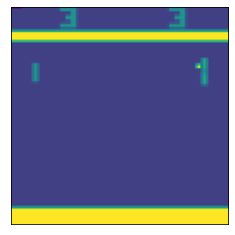
\includegraphics[width=0.32\linewidth]{images/Pong-Tfunc-good.png}}
  \subcaptionbox{Uncertain state\label{fig:subfig-b}}
    {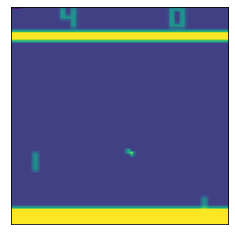
\includegraphics[width=0.32\linewidth]{images/Pong-Tfunc-normal.png}}
    \subcaptionbox{Dangerous state\label{fig:subfig-c}}
    {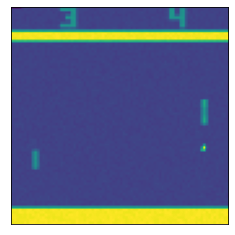
\includegraphics[width=0.32\linewidth]{images/Pong-Tfunc-bad.png}}
  \caption{Example of the behavior of the divergence function \(T\) for the game of Pong: the observation on the left (a) has a very low level of \(T\) since the probability that the agent fails is 0. The observation in the middle (b) presents a discrete \(T\) since considering the ball moving simply toward the right of the screen along the \(x\)-axis the agent can still make the ball bounce back. The third observation (c) has a very high value of \(T\) since there is no way the agent can save the ball.}
  \label{figure:t-func}
\end{figure}

\section{Results}
The next three sections show the {\it reward vs attack frequency curves} of all the evaluated policy attacks under a fixed threat model so to measure their effectiveness and their transferability against policies and algorithms. When analyzing the obtained results, sometimes we may refer to the curve of the policy attacked without transferability as baseline policy. In addition, we may sometimes intend as {\it attacking with a surrogate policy} or {\it attacking with a surrogate algorithm} as crafting adversarial perturbations exploiting a surrogate policy/algorithm to attack the target policy. Let's also remind that the purpose of these experiments is not only to evaluate the efficacy of different attack methods but to study their transferability proprieties. Hence, the relative value of each curve with respect to the other ones is more important than their individual absolute value.

\subsection{Attacking Pong-DQN}
The curves relative to this experiment are depicted in figure \ref{figure:pong-dqn}. We observe that in the case of uniform attack, the average rewards decrease from 20 to -20 almost linearly as the attack frequency increases from 0 to 0.5. For higher frequencies we didn't observe a larger drop in reward, thus meaning that the victim policy already performs close to the worst possible case. On the evaluated environment, uniform attack also shows good transferability both in terms of policy and algorithm. In particular, crafting adversarial observations with a similar policy yields similar results to attacking the baseline policy, obtaining almost identical performance for lower attack frequencies. Perturbations crafted on the other two algorithms, namely A2C and PPO, still successfully fool the victim agent with their curves following the trend of the baseline but maintaining an average reward difference of about 5 points.

Analyzing the curves relative to the strategically-timed attack, we can observe that the attack frequency is several grades of magnitude lower than uniform attack and is the lowest among all the examined policy attacks. In the frequency interval taken into consideration, which varies from 0.002 to 0.012, the corresponding average reward drops from a little more than 10 to less than -15 for the baseline policy which follows an almost linear decay. However, considering that this time adversarial observations are crafted in a targeted way, transferability seems to be less effective than it was for uniform attack. While attacking with policy transferability still yields results relatively closer to the baseline, perturbations crafted on the two on-policy algorithms often fail to fool the agent, thus requiring more attacks to provide meaningful results. 

Critical point attack has attack frequencies varying from 0.01 to 0.09, interval in which the reward falls from 20 to -15. As opposed to the previous two attacks, perturbations crafted under the surrogate policy don't work much better than the perturbations crafted on the policy trained with the other two on-policy attacks. Nevertheless, DQN policy transferability still seems to work a little better than A2C and PPO algorithm transferability as the attack frequency increases.
The curves of critical point and critical strategy attack are very similar both in terms of rewards and frequencies. However, both methods can't reduce the agent's reward to less than -15 in the given frequency interval. 

Finally, adversarial policy attack seems to perform the worst. The curves representing the two algorithms' transferability are very far from the other two curves and struggle to lower the reward to less than 10 points. The curve corresponding to policy transferability is also much weaker than the baseline but they follow the same trend and it is able to lower the average reward to less than 0 points. Overall, we can conclude saying that DQN is not a very robust algorithm since perturbations crafted with surrogate policies still fool the victim model with performance similar to directly attacking the victim policy. In fact, the closer are the curves to the baseline, the less robust is the target algorithm.

\begin{figure}
  \centering
  \subcaptionbox{Uniform attack \label{fig:subfig-a}}
    {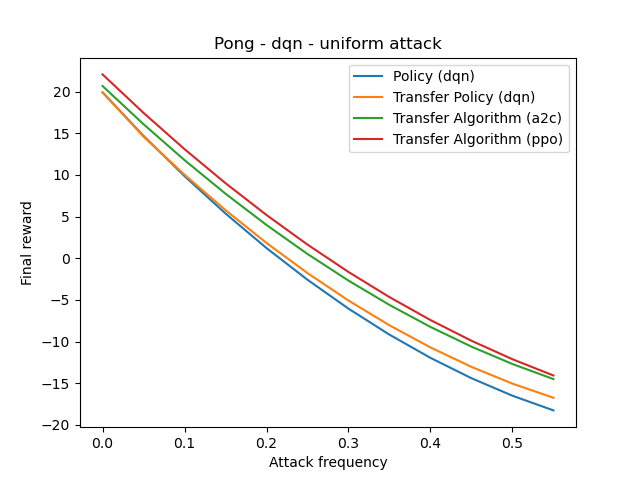
\includegraphics[width=0.49\linewidth]{images/exp1/dqn-pong-uniform.png}}
  \subcaptionbox{Strategically-timed attack\label{fig:subfig-b}}
    {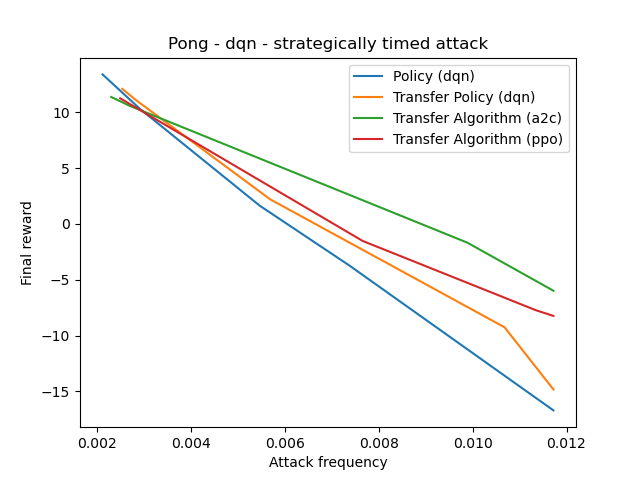
\includegraphics[width=0.49\linewidth]{images/exp1/dqn-pong-strategically_timed.png}}
  \subcaptionbox{Critical point attack\label{fig:subfig-c}}
    {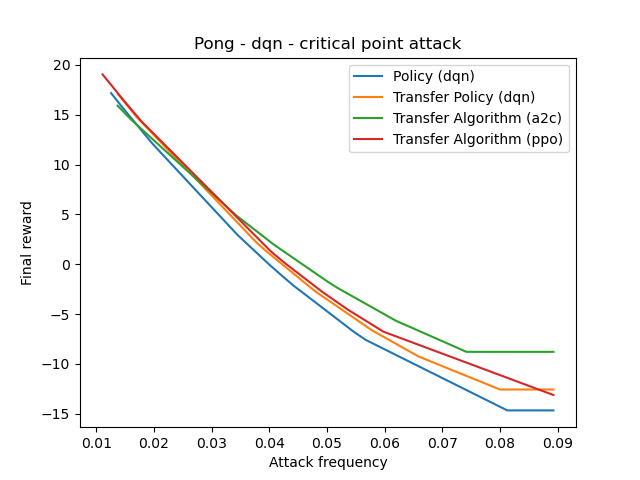
\includegraphics[width=0.49\linewidth]{images/exp1/dqn-pong-critical_point.png}}
  \subcaptionbox{Critical strategy attack\label{fig:subfig-d}}
    {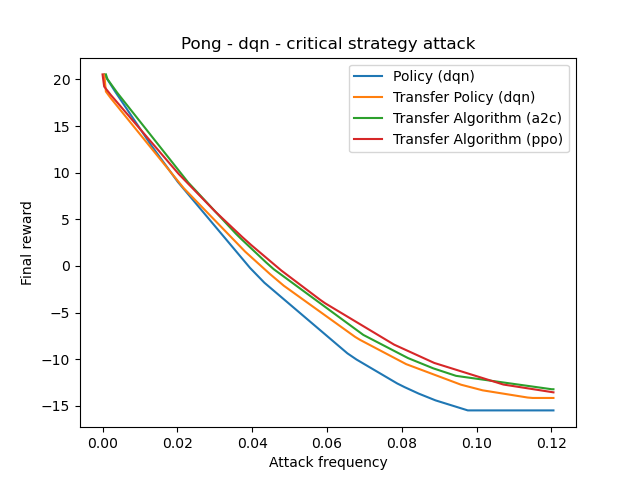
\includegraphics[width=0.49\linewidth]{images/exp1/dqn-pong-critical_strategy.png}}
  \subcaptionbox{Adversarial policy attack\label{fig:subfig-e}}
    {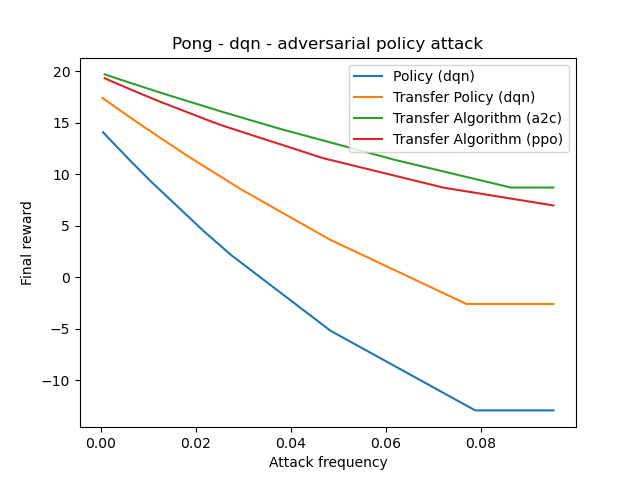
\includegraphics[width=0.49\linewidth]{images/exp1/dqn-pong-adversarial_policy.png}}
  \caption{The {\it reward vs. attack frequency} curves of 5 policy attacks with FGSM under the \(l_\infty\) norm attacking a Pong-DQN policy.}
  \label{figure:pong-dqn}
\end{figure}

\subsection{Attacking Pong-A2C}
The curves relative to the A2C policy are shown in figure \ref{figure:pong-a2c}. Beginning analyzing uniform attack, we can see that the curve of the baseline is similar to its corresponding DQN version but the performance of the surrogate policies drop considerably. Attacks with the surrogate similar policy still follow the trend of the baseline with a rapid decrease of the agent's reward for frequencies increasing from 0 to 0.25 and a more amortized decline until a frequency of 0.5. Attacks exploiting a surrogate algorithm never inflict too much damage in the considered interval with PPO producing the least effective perturbations. Adversarial observations crafted with DQN struggle to lower the average reward of the target policy to below 0 in the given frequency interval while PPO slowly reduces the rewards from 20 to 10. Strategically-timed attack once again benefits of a very low attack frequency. However, the robustness of A2C deeply impacts the effectiveness of the attacks with the surrogate policies. The baseline reduces the rewards from 20 to -15 attacking less than 2\% of the observed frames. Same as in uniform attack, adversarial examples generated attacking PPO need a higher attack rate to reduce the rewards by 10 points and DQN performs even worse. Also the baselines of the curves of critical point and critical strategy attack are similar to the baseline of their corresponding curves obtained in the previous section when attacking the DQN agent. As it was for the other methods, the surrogate policies perform much worse, with the attacks based on algorithm transferability suffering the most. Also in the case of adversarial policy, the adversary doesn't perform very well and its baseline resembles the one of uniform attack. In fact, it needs to increase the attack frequency to over 0.3 to achieve successful results. Attacks with DQN and PPO present very similar curves, both decreasing steadily to reduce the average reward to -5. We can then draw out the conclusion that A2C algorithm is more robust than DQN, in particular, it seems to resist very well against attacks with surrogate policies trained with different algorithms. In fact, all attacks show poor algorithm transferability and discrete policy transferability.

\begin{figure}


  \centering
  \subcaptionbox{Uniform attack\label{fig:subfig-a}}
    {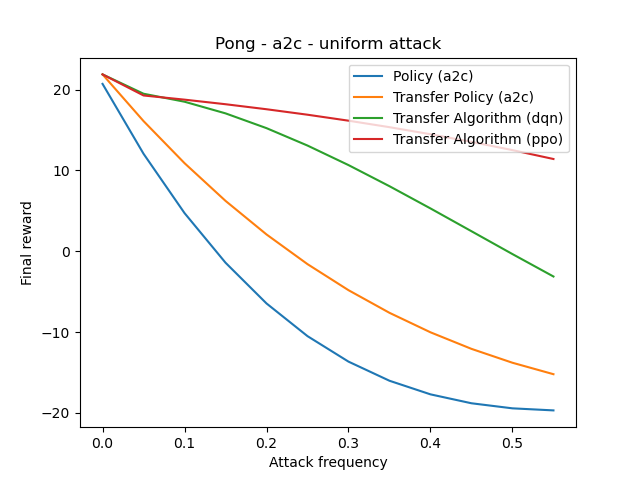
\includegraphics[width=0.49\linewidth]{images/exp1/a2c-pong-uniform.png}}
  \subcaptionbox{Strategically-timed attack \label{fig:subfig-b}}
    {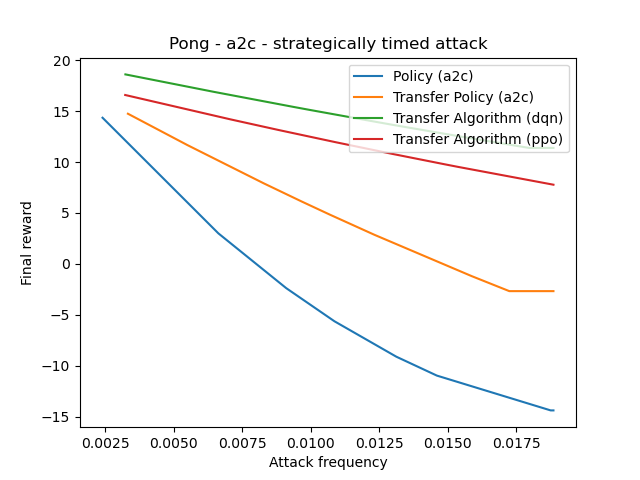
\includegraphics[width=0.49\linewidth]{images/exp1/a2c-pong-strategically_timed.png}}
  \subcaptionbox{Critical point attack\label{fig:subfig-c}}
    {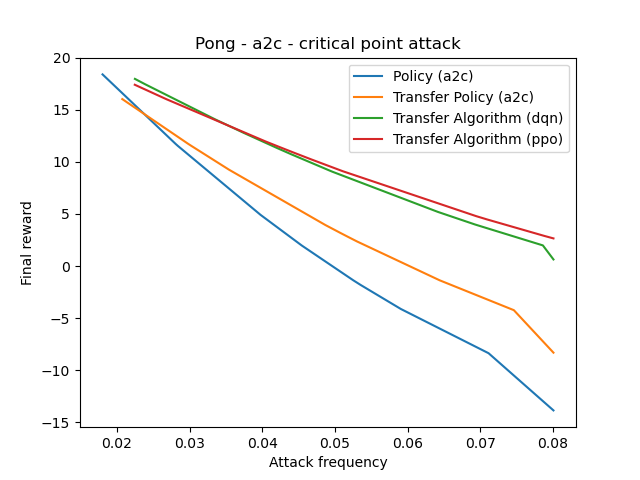
\includegraphics[width=0.49\linewidth]{images/exp1/a2c-pong-critical_point.png}}
  \subcaptionbox{Critical strategy attack\label{fig:subfig-d}}
    {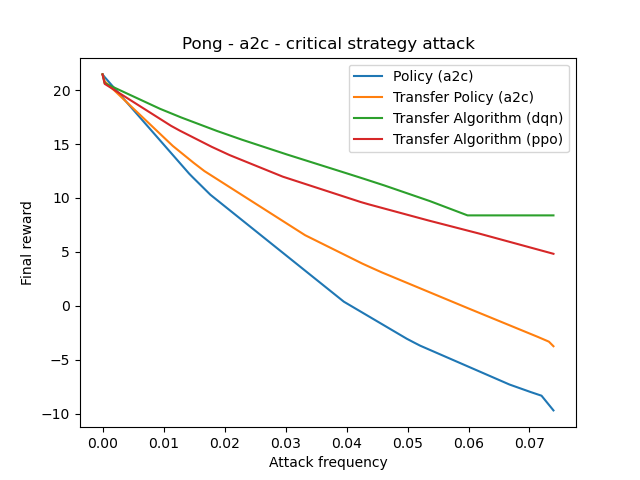
\includegraphics[width=0.49\linewidth]{images/exp1/a2c-pong-critical_strategy.png}}
  \subcaptionbox{Adversarial policy attack\label{fig:subfig-e}}
    {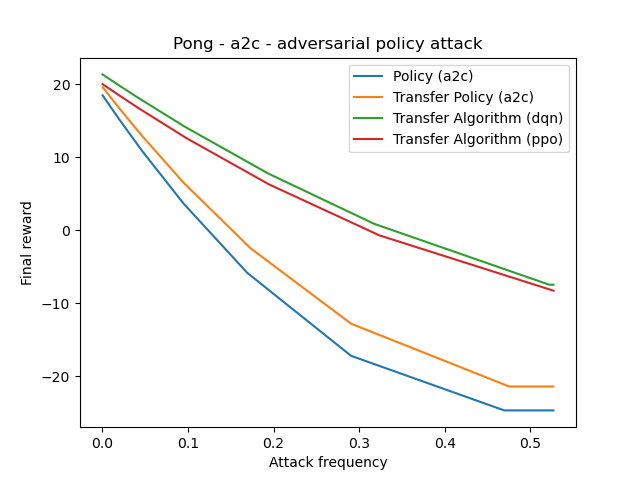
\includegraphics[width=0.49\linewidth]{images/exp1/a2c-pong-adversarial_policy.png}}
  \caption{The {\it reward vs. attack frequency} curves of 5 policy attacks with FGSM under the \(l_\infty\) norm attacking a Pong-A2C policy.}
  \label{figure:pong-a2c}
\end{figure}

\subsection{Attacking Pong-PPO}
The last set of charts depict the curves relative to the policy trained with PPO and it is shown in figure \ref{figure:pong-ppo}. Starting from the uniform attack, nothing new appears here with respect to the charts of the uniform attack relative to the other two algorithms. All curves follow the trend of the baseline but the adversarial examples generated with transferability are this time less effective. Attacks crafted with DQN are the ones performing the worst. Strategically-timed attack seems not to be able to attack as easily as it did against DQN. In fact, it requires a relatively higher attack frequency to achieve similar performance. Moreover, same as in the case of A2C, attacks with surrogate models trained with different algorithms, have to put more effort to decrease the average reward of the victim agent. Conversely, policy transferability still works discretely well. Critical point and critical strategy attack demonstrate good transferability and similar results, thus meaning that in the environment of Pong a hand-crafted divergence function is unnecessary to elaborate good attack strategies. Surprisingly, adversarial policy attack seems to work better than it did when attacking A2C. It can almost linearly lower the agent's average reward from 20 to 0 attacking no more than 20\% of the frames. and it also owns a better transferability property than it had against A2C and DQN. Overall, PPO seems to be a little more robust than DQN but less robust than A2C. In terms of transferability all attacks, except for strategically-timed attack, are able to craft effective adversarial observations using their respective surrogate policies. Strategically-timed attack still works very well under policy transferability but fails when attacking with different algorithms.

\begin{figure}
  \centering
  \subcaptionbox{Uniform attack \label{fig:subfig-a}}
    {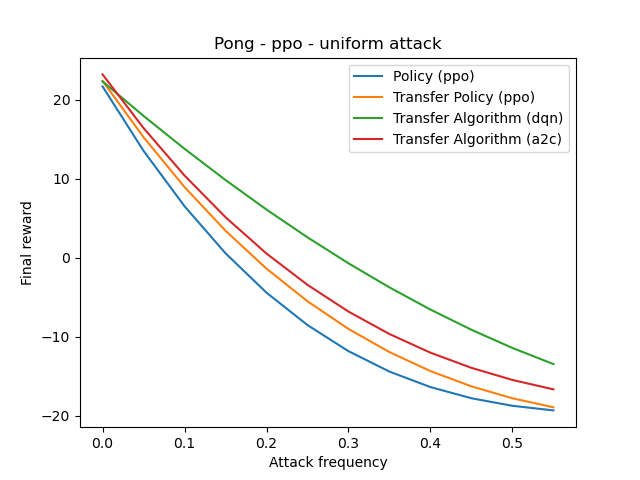
\includegraphics[width=0.49\linewidth]{images/exp1/ppo-pong-uniform.png}}
  \subcaptionbox{Strategically-timed attack\label{fig:subfig-b}}
    {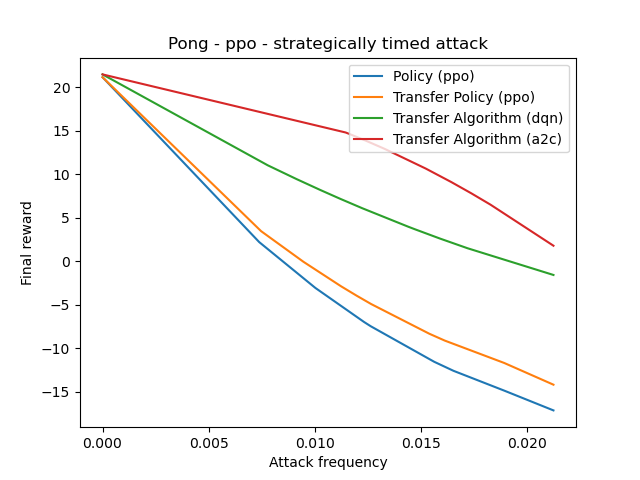
\includegraphics[width=0.49\linewidth]{images/exp1/ppo-pong-strategically_timed.png}}
  \subcaptionbox{Critical point attack\label{fig:subfig-c}}
    {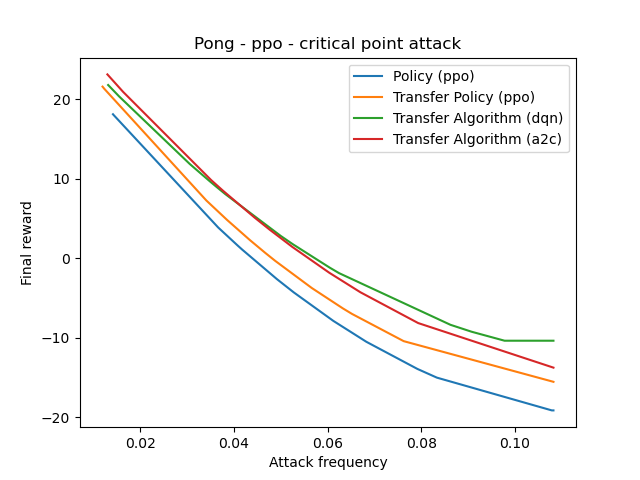
\includegraphics[width=0.49\linewidth]{images/exp1/ppo-pong-critical_point.png}}
  \subcaptionbox{Critical strategy attack \label{fig:subfig-d}}
    {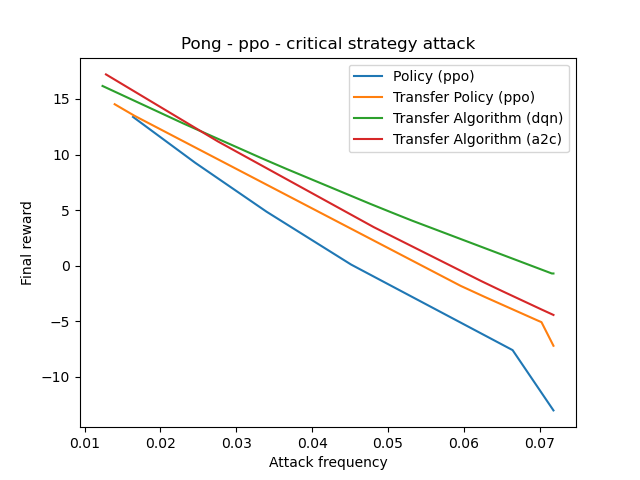
\includegraphics[width=0.49\linewidth]{images/exp1/ppo-pong-critical_strategy.png}}
  \subcaptionbox{Adversarial policy attack \label{fig:subfig-e}}
    {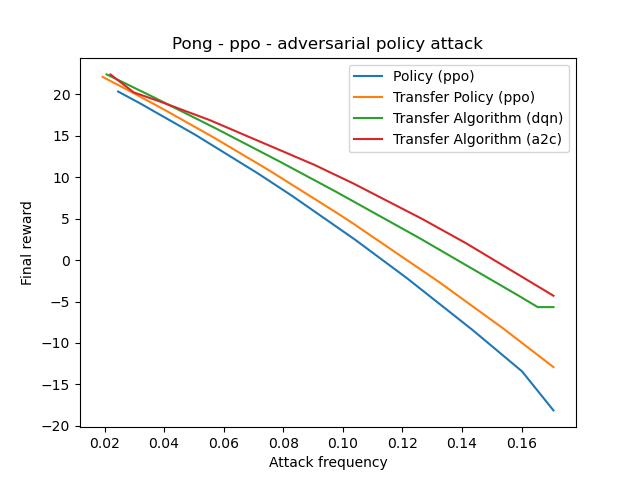
\includegraphics[width=0.49\linewidth]{images/exp1/ppo-pong-adversarial_policy.png}}
  \caption{The {\it reward vs. attack frequency} curves of 5 policy attacks with FGSM under the \(l_\infty\) norm attacking a Pong-PPO policy.}
  \label{figure:pong-ppo}
\end{figure}

\section{Findings}
This section analyses the policy attack methods that have been evaluated in this experiment and draws some conclusions about their usage, effectiveness, and drawbacks. It also points out some future research directions to improve those attacks and makes insightful comparisons among similar methods.

\subsection{Uniform attack vs strategically-timed attack}
Not surprisingly, uniform attack is the most simple but also the weakest attack that has been examined in the present evaluation. However, it is very fast and is compatible with untargeted image attacks, thus allowing the exploration of other image attacks such as Deepfool that only work under untargeted settings \cite{moosavidezfooli2016deepfool}. Interestingly, strategically-timed attack achieves the best performance under the lowest frequencies. The reason behind its excellent performance is that this method has specifically been designed to work under low attack frequencies attacking only in correspondence with the most critical observations. Being its attacks very sparse, it takes more frames to make the victim agent fail. Hence, resulting in a very low attack frequency. The intelligent way strategically-timed attack decides whether to attack an observation or not could be also borrowed to other methods such as uniform attack to lower their frequency while limiting the drop in performance. In this work, this technique has been applied also to the adversarial policy attack to vary its frequency. One possible drawback of this technique is that it may miss some observations that apparently don't seem critical but that attacking them may lead to worse states in the future steps, a drawback that has more important consequences in the case of the adversarial policy attack.

\subsection{Critical point vs critical strategy attack}
Critical point attack and critical strategy attack are constrained by the hyper-parameter \(n\) which, forcing the two methods to attack every observation over sequences of \(n\) frames, might result in some unnecessary attacks. Overall, the attack frequency is largely influenced by the \(m\) parameter which defines the number of steps taken without attacking the policy of the agent. Higher values of \(m\) comport a decrease of the attack frequency but also lead to a potential risk of missing some critical states which it would have been worth attacking. In fact, the last \(m-n\) observations of an observed trajectory are completely ignored by both attacks. Different frequencies are thus generated varying \(n\) and \(m\). Going more deeply into understanding their behaviors, critical point attack relies on a divergence function to estimate how critical is the last state of a trajectory defined by a strategy. However, both the strategy that defines some sequences of malicious actions and the divergence function of critical point attack are hand-crafted, which means that they require some domain knowledge to be designed by a human. While a strategy that works for a certain environment may still work quite well in similar environments, a specific divergence function will not work in other environments, even for similar ones. For instance, a strategy that only repeats the same action is considered a malicious strategy for almost all the Atari environments, but clearly, this transferability property may not be true for some other environments. In contrast, critical strategy attack depends on the cumulative reward over a trajectory to determine the maliciousness of a strategy: the lower the reward the more malicious a strategy is. However, what makes reinforcement learning challenging is exactly the sparsity of the rewards. This means that the value of most trajectories will be zero. On one hand, this is a positive property since adversarial strategies will always aim to prevent the agent to increase its score, eventually leading it to fail the episode or lose one life. On the other hand, with many strategies preventing the agent to get any reward along, it's not easy to determine which one may continue to lead the agent to more malicious states in the future steps. For both attacks, the special case where \(m=n\) means attacking every frame and both attacks are more effective as \(n\) increases and the difference \(|m-n|\) reduces. Furthermore, the hyper-parameter \(n\) has influence on the number of adversarial strategies to be tested. Supposing \(a\) to be the number of actions of an environment and the strategies to be all possible combinations of \(n\) actions, \(a^n+a*(m-n)\) strategies will be evaluated with \(n\) adding an exponential computational cost since more strategies will be evaluated. Thus, the way to generate adversarial strategies should be carefully crafted. Overall, critical point attack performs slightly better than critical strategy but it depends on a divergent function to be computed on the input observations which sometimes could be a challenging task.

\subsection{Adversarial policy and future search directions}
Given the results presented in this section, apparently adversarial policy attack is the one performing the worst. The reason behind this is that this method doesn't have a real mechanism to control and vary its frequency. Hence, it borrows the technique used by strategically-timed attack. The difference between the two is that while the strategically-timed attack executed the least likely action, adversarial policy attack crafts perturbations such that the victim agent executes a specific action predicted by the network implementing the adversarial policy. In fact, in adversarial policy attack, all actions are equally important since the goal here is to lead the agent toward a certain state where failure is inevitable. However, missing one or a few steps because wrongly considered as not critical may lead to other less malicious policies. Generally, this method as well as critical point and critical strategy, focuses on making the agent fail faster rather than slowly sabotage it as uniform attack and strategically-timed attack do. However, blindly attacking each frame is still not an elegant solution to make these attacks effective. Attacking more observations not only requires more computational power but also increases the possibility of the attacker being detected. If hand-crafting a mechanism to determine when to attack is not enough for such more complex methods, then machine learning is once again the answer. Future research directions might then focus also on {\it when to attack} rather than {\it how to attack}, thus learning to predict critical observations along the corresponding malicious action and even learning to limit the number of attacks so to control the frequency. \cite{sun2020stealthy} pioneers this work with antagonist attack.

\subsection{Attack feasibility in common scenarios}
Another point that is important to mention is that strategically-time attack takes advantage of the logits or probability of the predicted actions in order to attack the victim agent. However, this knowledge is not always available under common threat models. Thus, although the above-mentioned attack seems to work extremely well under experiment settings, in practice it may result ineffective in real-world scenarios. In contrast, to use uniform attack the adversary only needs to know the action predicted by the model representing the policy so to cause it to take another random action. This knowledge is usually more commonly available than the actions probabilities but it is still a limiting constraint to make the attack work. However, this contrast could be relaxed by assuming the target agent to have taken a certain action, even a random action, and consequently use it to craft the corresponding perturbations. Critical point and critical strategy both need a simulator of the environment to assert the value of their strategies. In the best-case scenario, a copy of the state of the environment could be used so as to exactly know the outcome of each strategy. In fact, both methods could take actions in the environment according to the actions defined in a strategy, compute the value of the last observation or the value of the trajectory and then revert it to the saved state so to evaluate the next strategy. If retrieving the state of the environment is not possible, then it should be engineered other ways to make a simulation of the environment that is as close as possible to the original one. The authors of critical point attack proposed to train a neural network that given an observation and an action it predicts the next observation. An interesting solution is the one introduced in \cite{kim2020learning} which trains a variant of GAN to learn a simulator by simply watching an agent interact with the environment. In those circumstances where, for any reason, a simulation of the environment is not available, attack strategies can still be computed based on a simulation of similar environments or simply designing some strategies that intuitively may be malicious for the target environment regardless of its current state. The only requirement adversarial policy attack needs in order to attack its target is to have access to the input observations. Therefore, this method is more flexible since it can work under different threat models. However, it still needs to be trained in the same environment of the victim policy before it can be used to attack it. Let's remind that all the policy attacks evaluated in this thesis work only under the condition that input observations can be modified. Table \ref{table:atk_req} summarizes the requirements of each policy attack to work properly.

\begin{table}
  \centering
  \caption{Requirements needed for each evaluated policy attack method to work properly.}
  \begin{tabular}{ccccc}
    \toprule
    Attack method & Observations & Environment & Pred action & Actions probs              \\
    \midrule
     Uniform Attack & V & - & V & - \\ 
 Strategically-Timed Attack & V & - & - & V \\
 Critical Point Attack & V & V & - & - \\
 Critical Strategy Attack & V & V & - & - \\
 Adversarial Policy & V & Only for training & - & - \\
    \bottomrule
  \end{tabular}
  \label{table:atk_req}
\end{table}

\subsection{Online vs offline attacks}
Uniform attack, strategically-timed attack, and adversarial policy attack are relatively fast attacks. In fact, excluding the time the image attack method takes to generate the adversarial perturbations, the first two methods only involve a few linear computations while the third one requires one forward pass of its network. Hence, those three attacks, combined with a fast image attack method, are suitable to attack in an online way following the stream of states observed by the target agent. Conversely, critical point and critical strategy attack need to explore and assert the damage of different strategies before start attacking and this operation should be repeated every \(n+m\) frames. This bottleneck makes these two attacks too slow to be executed in an online way but more useful to attack offline when time is not a constraint. Nevertheless, in real life scenario is more common to have to attack online rather than offline.
\chapter{STUDYING POLICY ATTACKS TRANSFERABILITY AGAINST DEFENDED POLICIES}
\label{sec:exp2}

This section reports the results of the second of the three experiments included in this thesis. It evaluates the same policy attacks but this time attacking defended policies. It still focuses on attacks' transferability and shows some interesting findings

\section{Studying policy attacks transferability against defended policies}
This experiment can be viewed as the direct extension of the previous one showed in section \ref{sec:exp1}. This time, all the policies under attack have been defended with FGSM adversarial training and the goal of this work is to study the transferability of some policy attack methods against defended policies. To draw the {\it reward vs accuracy} curve of the evaluated methods, adversarial training has been conducted with a value of \(epsilon\) slightly inferior to the \(epsilon\) that defines the distance of the adversarial perturbations. In this way, it's more clear the effect of the attacks against the defended policies. The experiments have been conducted on the same three reinforcement learning algorithms adopted in section \ref{sec:exp1}: DQN, A2C, and PPO with policies trained only on the environment of Pong. In addition, the policy attack methods that have been compared include:
\begin{itemize}
    \item Uniform attack;
    \item Strategically-timed attack.
\end{itemize}
The reason why we have chosen only uniform attack and strategically-timed attack is to test one method based on untargeted image attacks and the second one based on targeted image attacks. Given the previous results, these two methods are enough to have a general idea of the robustness of an algorithm. Thus, the scope of the experiment has then been reduced to 2 policy attacks.

\subsection{Experiments settings}
\subsubsection{Defenses hyper-parameters}
\label{sec:exp2-params}
All policies have been protected with FGSM adversarial training applied over the same policies trained normally. This means that adversarial training has not been applied on models training from scratch but it has been applied on models that had already learned a working policy. Once again, FGSM has been chosen because of its speed over iterative methods. Many works such as \cite{li2020understanding} cite that during FGSM adversarial training, the robust accuracy of the model would suddenly drop to almost 0\% after a certain point. This phenomenon was commonly referred to as {\it catastrophic overfitting}. The reason for this phenomenon is that, since FGSM is a simple attack, the model learns to fool the FGSM attacks by inducing obfuscated gradient, thus making the gradient no longer a useful direction for constructing adversarial examples. However, the way adversarial training is applied to reinforcement learning algorithms is a little different from the standard adversarial training applied to image classification models and not much is known about catastrophic overfitting under reinforcement learning adversarial training. The second important point to remark is that during adversarial training perturbations have been crafted with \(epsilon=0.01\) and, when attacking, policies' noise \(epsilon\) has been raised to 0.05. All distances are computed under \(l_\infty\) norm. This discrepancy is to make sure that the adversarial perturbations can break the defended policies so as to draw more understandable {\it reward vs attack frequency} curves. As we can see from table \ref{table:adv_def}, adversarial training works well enough that adversarial observations crafted with the same perturbation distance used during training are not capable to fool the defended model. Moreover, the configuration of the algorithms during adversarial training is the same used in the previous experiments. The only small difference regards DQN, since the base policy has already been trained, the algorithm doesn't need much exploration during adversarial training. Consequently, the exploration noise has been held fixed to 0.05 for the whole process of training. The training process has been conducted over 2.5M frames for DQN and 5M frames for A2C and PPO. During adversarial training, the network is given in input adversarial observations with probability 0.5 and clean observations with the same probability so as to not forget how to deal with clear observations. In another experiment where adversarial training was conducted only using adversarial observation, the trained policy worked very well in presence of perturbations but seemed to predict random actions in correspondence to clear observations.

\begin{table}
  \centering
  \caption{Average reward scored by three policies trained with DQN, A2C and PPO respectively and defended with FGSM Adversarial training with \(epsilon=0.01\) under \(l_\sameinfty\) norm.}
  \begin{tabular}{cccc}
    \toprule
    Observations & DQN (FGSM-AT) & A2C (FGSM-AT) & PPO (FGSM-AT) \\
    \midrule
     Clear & 19.6 & 18.8 & 19.7 \\ 
     Adversarial & 19.4 & 17.9 & 18.7 \\
    \bottomrule
  \end{tabular}
  \label{table:adv_def}
\end{table}

\subsubsection{Image adversarial attacks settings}
The configuration of the white-box attacks is identical to the one used in the previous experiment in section \ref{sec:exp1}. In this way, we provide a fair comparison with the curves obtained when attacking undefended policies.

\section{Results}
The next two sections show the {\it reward vs. attack frequency} curves of uniform attack and strategically-timed attack under a fixed threat model so to measure their effectiveness and their transferability against policies and algorithms protected with adversarial training. When analyzing the obtained results, sometimes we may refer to the curve of the policy attacked without transferability as baseline policy. In addition, we may sometimes intend as attacking with a surrogate policy or attacking with a surrogate algorithm as crafting adversarial perturbations exploiting a surrogate policy/algorithm to attack the target policy. Since we want to focus on studying attack transferability and that the adversary is cheating by crafting perturbations that are stronger than the ones crafted by adversarial training, we will ignore the absolute performance of the curves but we will focus on their relative distance between each other and the baseline. In fact, table \ref{table:adv_def} shows that, even if all observations were adversarial, that is when the attack frequency is equal to 1, crafting adversarial observations with the same perturbation strength used during training the average reward wouldn't be lowered too much respect to not performing any attack at all.

\subsection{Attacking adversarially trained Pong-DQN}
The curves obtained attacking Pong-DQN with uniform and strategically-timed attack are shown in figure \ref{figure:pong-dqn-def}. The first thing we can observe is that the curves of the baseline and of the surrogate policy are practically identical, this indicates that uniform attack benefits an excellent policy transferability. Similarly, also the curve for the algorithm transferability of A2C stays close to the baseline, thus showing a good transferability. This phenomenon is more clear in correspondence to higher attack frequencies. Only attacks crafted with PPO seem to be less capable to fool the target policy. In fact, its corresponding curve keeps a distance of about 10 points with respect to the baseline in the evaluated frequency interval. Analyzing strategically-timed attack, we can surprisingly note that attacking with the surrogate policy yields even better results than directly attack the target policy. Overall, PPO is the worst algorithm when crafting adversarial perturbations and it is always a safer choice to craft them on a policy trained with the same algorithm. 

\begin{figure}
  \centering
  \subcaptionbox{Uniform attack\label{fig:subfig-a}}
    {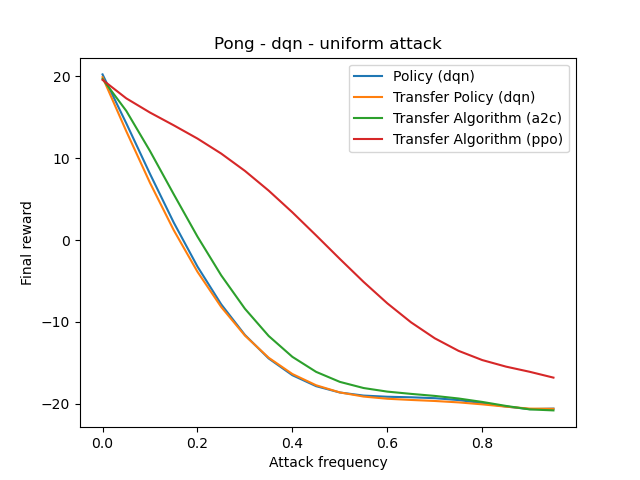
\includegraphics[width=0.49\linewidth]{images/exp2/dqn-pong-uniform.png}}
  \subcaptionbox{Strategically-timed attack\label{fig:subfig-b}}
    {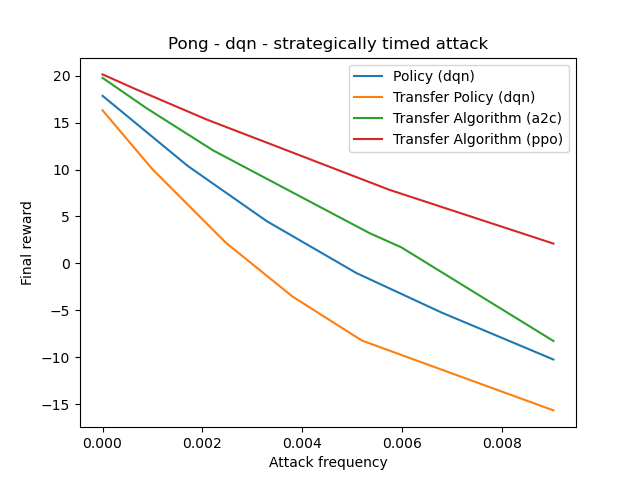
\includegraphics[width=0.49\linewidth]{images/exp2/dqn-pong-strategically_timed.png}}
  \caption{The {\it reward vs. attack frequency} curves of 2 policy attacks with FGSM under the \(l_\infty\) norm attacking a Pong-DQN policy defended with FGSM adversarial training with \(epsilon=0.01\). Attacks have been performed with \(epsilon=0.05\) to show the drop in reward as the attack frequency increases.}
  \label{figure:pong-dqn-def}
\end{figure}

\subsection{Attacking adversarially trained Pong-A2C}
The curves resulting from attacking Pong-A2C are depicted in figure \ref{figure:pong-a2c-def}. The chart presents a similar pattern to the chart of the corresponding DQN version. In fact, the curves relative to policy transferability and DQN algorithm transferability remain close to the baseline. Attacks crafted on PPO result to be less effective with its curve remaining about 5 points over the other curves. Regarding strategically-timed attack, the curve of the surrogate A2C policy is still very close to the baseline of A2C. In this case, the perturbations crafted on DQN are the ones that perform the worst followed by A2C but still maintaining only a few points of difference with respect to the baseline. 

\begin{figure}
  \centering
  \subcaptionbox{Uniform attack\label{fig:subfig-a}}
    {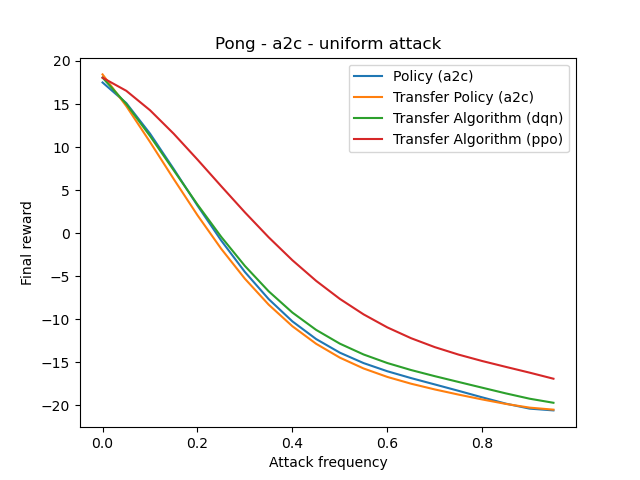
\includegraphics[width=0.49\linewidth]{images/exp2/a2c-pong-uniform.png}}
  \subcaptionbox{Strategically-timed attack\label{fig:subfig-b}}
    {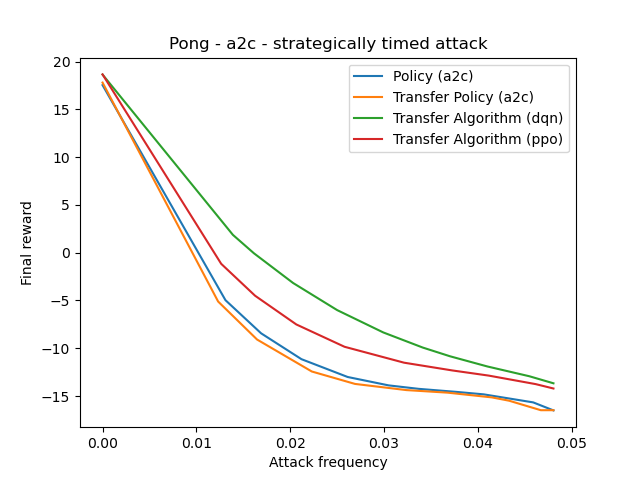
\includegraphics[width=0.49\linewidth]{images/exp2/a2c-pong-strategically_timed.png}}
  \caption{The {\it reward vs. attack frequency} curves of 2 policy attacks with FGSM under the \(l_\infty\) norm attacking a Pong-A2C policy defended with FGSM adversarial training with \(epsilon=0.01\). Attacks have been performed with \(epsilon=0.05\) to show the drop in reward as the attack frequency increases.}
  \label{figure:pong-a2c-def}
\end{figure}

\subsection{Attacking adversarially trained Pong-PPO}
The curves obtained from attacking Pong-PPO are represented in figure \ref{figure:pong-ppo-def}. Attacks crafted with any policy show a good transferability for the uniform attack such that choosing any surrogate model to generate adversarial observations would yield performance similar to attacking the victim model. PPO policy is a little more robust against strategically-timed attack which presents more spaced curves. More specifically, transferability over A2C works better than transferability over DQN, and transferability over PPO is the one that yields performance most similar to the baseline.

\begin{figure}
  \centering
  \subcaptionbox{Uniform attack\label{fig:subfig-a}}
    {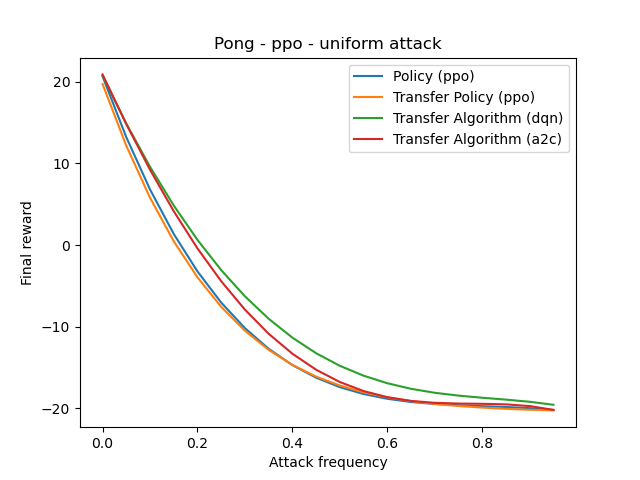
\includegraphics[width=0.49\linewidth]{images/exp2/ppo-pong-uniform.png}}
  \subcaptionbox{Strategically-timed attack\label{fig:subfig-b}}
    {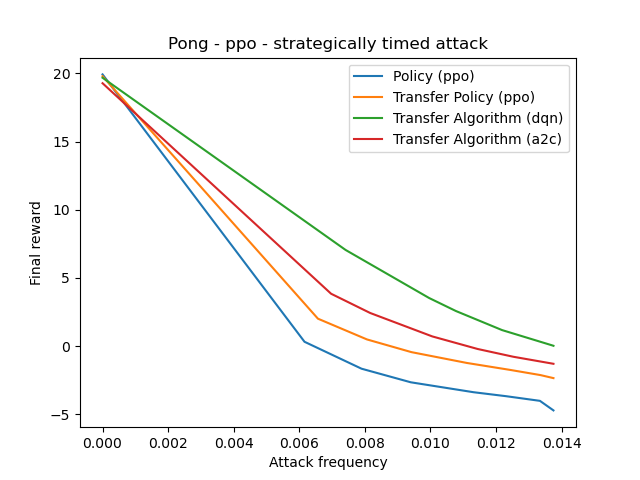
\includegraphics[width=0.49\linewidth]{images/exp2/ppo-pong-strategically_timed.png}}
  \caption{The {\it reward vs. attack frequency} curves of 2 policy attacks with FGSM under the \(l_\infty\) norm attacking a Pong-PPO policy defended with FGSM adversarial training with \(epsilon=0.01\). Attacks have been performed with \(epsilon=0.05\) to show the drop in reward as the attack frequency increases.}
  \label{figure:pong-ppo-def}
\end{figure}

\section{Findings}
This section provides further analyses about the policies that have been evaluated. In particular, it makes some conclusions about the performance obtained when attacking with similar policies and with similar algorithms.

\subsection{Performance of similar policies}
In most of the charts showed in this section as well as in section \ref{sec:exp1}, the attacks crafted on the surrogate policies trained with the same algorithm of the victim policy own a better transferability than the attacks crafted on the policies trained with different algorithms. We can then conclude that attacking similar policies is more effective than attacking different algorithms. This is the same property observed when attacking common image classificators: attacking a surrogate model with the same architecture provides better results than attacking models with different architectures.

\subsection{Performance of similar algorithms}
Among the three evaluated algorithms, DQN is off-policy, which means that it learns in a different way than A2C and PPO which are on-policy. Moreover, A2C and PPO are substantially similar with the introduction of the clipping hyper-parameter being a major difference. Hence, as we can see from the charts of the experiments in both this chapter and in the previous one, a policy trained with A2C can be more easily attacked with PPO rather than with a policy trained with DQN. On the other way around, a policy trained with PPO can be more easily attacked with A2C. Thus algorithm transferability is more effective when the surrogate policy is trained with an algorithm similar to the algorithm used to train the victim policy.
\chapter{BENCHMARK OF EFFECTIVENESS OF IMAGE ATTACK METHODS AGAINST DEFENDED POLICIES}
\label{sec:exp3}

This section reports the results of the last of the three experiments included in this thesis. It benchmarks the effectiveness of different image attacks used by two different policy attacks to decrease victim's rewards. The victim models have been protected with different defense mechanisms. 

\section{Benchmark of the effectiveness of image attack methods against defended policies}
The last experiment included in this work consists of a benchmark to evaluate the robustness of defended policies trained with DQN on the environment of Pong. All policies have been attacked with the white-box image attack FGSM under a fixed threat model. This work compares the {\it reward vs perturbation} and {\it accuracy vs perturbation} curves of the defended victim policies by attacking them over increasing values of perturbations’ strength. Policies have been defended with the following defense methods:
\begin{itemize}
    \item FGSM adversarial training;
    \item PGD adversarial training;
    \item JPEG conversion;
    \item Feature squeezing (Bit squeezing);
    \item No defense.
\end{itemize}
Note that in the benchmark is also included an undefended version of the victim policy so as to have a comparison of the defended policies with the undefended one. 
Policies have been attacked with three different white-box image attacks methods including:
\begin{itemize}
    \item FGSM;
    \item PGD;
    \item MI (Momentum Iterative);
    \item No attack.
\end{itemize}
The {\it no attack} method which corresponds to evaluating the target policy without attacking it at all has been introduced so to compare the effect of each attack method with respect to not attacking at all. The curves have been generated attacking with both untargeted and targeted attacks and their corresponding results are reported in two different sections.

\subsection{Experiments settings}
\subsubsection{Defenses hyper-parameters}
Two of the four defenses that have been included in the benchmark consist of adversarial training with FGSM and PGD respectively. The first policy is the same policy trained with DQN used in the experiment in section \ref{sec:exp2}. The policy protected with PGD adversarial training has been trained crafting adversarial perturbations with 10 iterations of PGD. Besides the type of attack and the number of iterations, there is no difference between the way adversarial training has been applied. Perturbations have been crafted under \(l_\infty\) norm and \(\epsilon\) fixed to 0.01. 

The third defense that has been implemented is a simple method that converts each observation to JPEG format before feeding it to the network. JPEG images retain 20\% of the quality of the original observations. 

The fourth method is known as feature squeezing and it consists of reducing the number of features of each pixel for each observed image. Since we are dealing with gray-scale images, what we are going to reduce is the number of bits to represent each pixel, thus we may sometimes refer to this method as bit squeezing. More specifically, it reduces the number of bits from 8 to 5, thus lowering the number of features from \(2^8\) to \(2^5\). This method shrinks the number of features by 80\% with respect to the original observations.

In this benchmark we have evaluated a powerful defense method such as adversarial training and two simple defenses such as JPEG conversion and feature squeezing so to test defenses with different levels of effectiveness.

\subsubsection{Image adversarial attacks settings}
This section reports the value of the hyper-parameters adopted in the image attacks included in the benchmark. Note that this time the perturbation strength \(epsilon\) is variable. The first attack, FGSM, has already been employed in the previous experiments and its hyper-parameters are maintained the same for this work. The two iterative methods PGD and MI execute 10 iterations each attack and each iteration refines the adversarial perturbations with \(epsilon_i\) (attack step size) of \(\epsilon/5\). 

The main reason why we have chosen the above-mentioned attacks is that they all work under targeted and untargeted settings and they support the three most common distance norms, namely \(l_\infty, l_1, l_2\). They also explicitly define the hyper-parameter \(\epsilon\) to limit the size of the adversarial perturbations. For example, adversarial examples crafted with C\&W method are not easily comparable in this benchmark since the method doesn't have a hyper-parameter \(\epsilon\) that can be fine-tuned. Moreover, those attacks are well-studied and commonly used in research papers, thus proving to work well in practice and worth being evaluated.

\subsubsection{Threat model}
All methods included in this benchmark are evaluated under both untargeted and targeted settings. Adversarial examples are crafted using the \(l_\infty\) distance norm. Their perturbations' strength \(\epsilon\) ranges from 0 to 0.05 included with a step size of 0.005. Curves are generated by computing the rewards of the policy under attack and the success rate of the malicious attacks according to the value of \(\epsilon\) defined in correspondence of each point.

\subsection{Benchmark of untargeted white-box attacks}
The charts relative to the {\it reward vs perturbation} and {\it accuracy vs perturbation} curves obtained under untargeted settings are shown in figures \ref{figure:untargeted-rew} and \ref{figure:untargeted-suc} respectively. When attacking the policy protected with FGSM adversarial training, MI is the attack that results most effective followed by PGD and FGSM. It is interesting to note that although adversarial training has been conducted with \(\epsilon\)=0.01, adversarial training can still protect quite well against adversarial observations crafted with higher values of perturbation strength. The defense is completely broken for noise generated with \(\epsilon\) greater than 0.03. Conversely, when attacking PGD adversarial training, FGSM and PGD perform the best but the difference between the three attack methods is never too significant. PGD struggles to reduce the reward of the agent against JPEG filter and bit squeezing with respect to the other two attack methods which perform very similar. FGSM is also the only attack that can't reduce the average reward to \(-20\) when attacking the undefended policy. When comparing the success rate of the three methods, PGD is the attack the overall performs the best and FGSM is the worst. In particular, PGD adversarial training seems to be more robust against FGSM, and bit squeezing is more vulnerable against PGD attack. When attacking FGSM adversarial training and JPEG filer, all the attacks show a similar success rate.

It is interesting to note that when attacking JPEG filter and bit squeezing, all attacks seem to break the defense right after increasing the strength of the perturbations to be greater than 0.01. In fact, after this threshold, their curves drop to -20 points and the attack accuracy skyrockets to be 100\%. The two defenses based on adversarial training are better at improving the robustness of their policies. As we can see from the charts, the average rewards still begin decreasing when \(\epsilon\) is greater than 0.02 or 0.03 but both curves approach -20 with a more gentle descent. Conversely, the attack accuracy against the same defenses steadily increases over the whole perturbations range but the rise is never too steep.


\begin{figure}
  \centering
  \subcaptionbox{FGSM adversarial training\label{fig:subfig-a}}
    {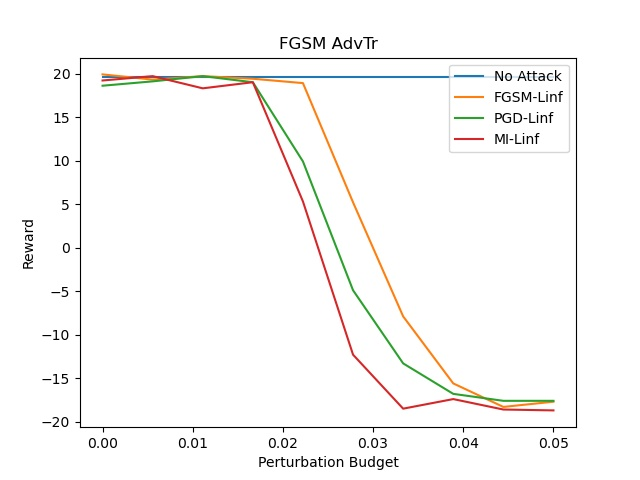
\includegraphics[width=0.49\linewidth]{images/exp3/untargeted/FGSM_AdvTr.jpg}}
  \subcaptionbox{PGD adversarial training\label{fig:subfig-b}}
    {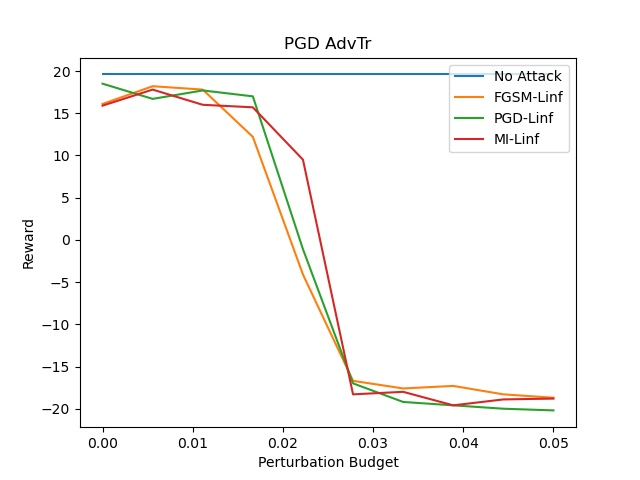
\includegraphics[width=0.49\linewidth]{images/exp3/untargeted/PGD_AdvTr.jpg}}
  \subcaptionbox{JPEG filter\label{fig:subfig-c}}
    {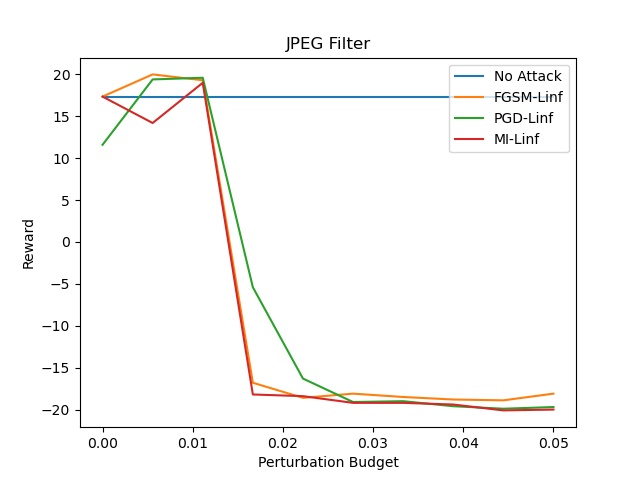
\includegraphics[width=0.49\linewidth]{images/exp3/untargeted/JPEG_Filter.jpg}}
  \subcaptionbox{Bit squeezing\label{fig:subfig-d}}
    {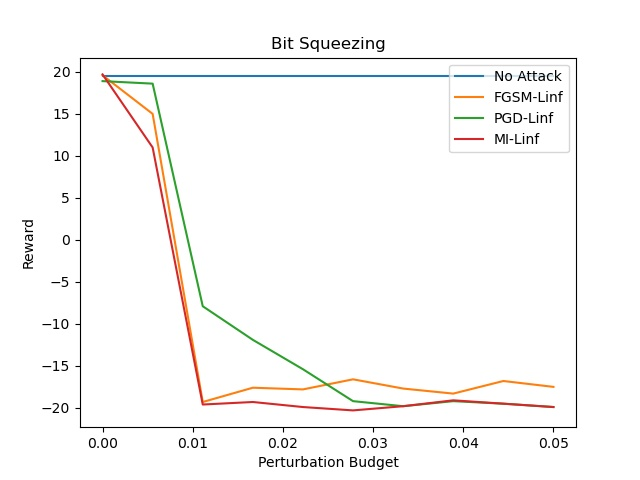
\includegraphics[width=0.49\linewidth]{images/exp3/untargeted/Bit_Squeezing.jpg}}
  \subcaptionbox{No Defense\label{fig:subfig-e}}
    {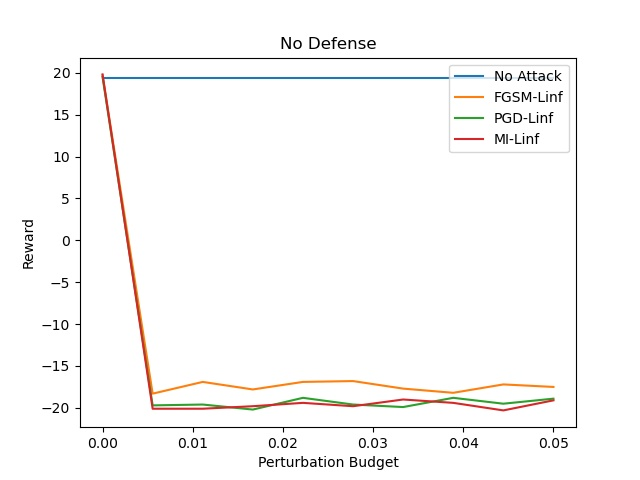
\includegraphics[width=0.49\linewidth]{images/exp3/untargeted/No_Defense.jpg}}
  \caption{The {\it reward vs perturbation} curves of 5 DQN policies trained to play Pong and defended with 5 different defense methods (including no defense) under the \(l_\infty\) norm attacking with increased perturbations strength. Perturbations have been crafted in an untargeted way.}
  \label{figure:untargeted-rew}
\end{figure}

\begin{figure}
  \centering
  \subcaptionbox{FGSM adversarial training\label{fig:subfig-a}}
    {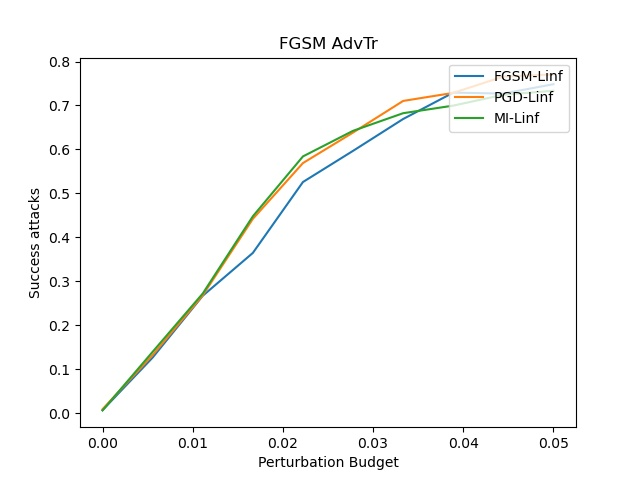
\includegraphics[width=0.49\linewidth]{images/exp3/untargeted/FGSM_AdvTr_succ.jpg}}
  \subcaptionbox{PPO adversarial training\label{fig:subfig-b}}
    {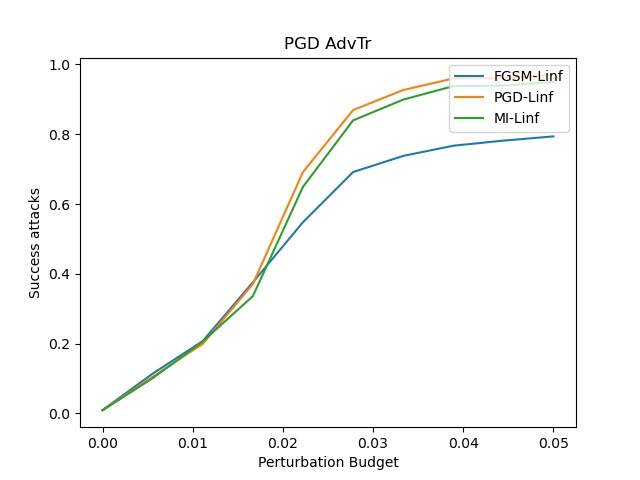
\includegraphics[width=0.49\linewidth]{images/exp3/untargeted/PGD_AdvTr_succ.jpg}}
  \subcaptionbox{JPEG filter\label{fig:subfig-c}}
    {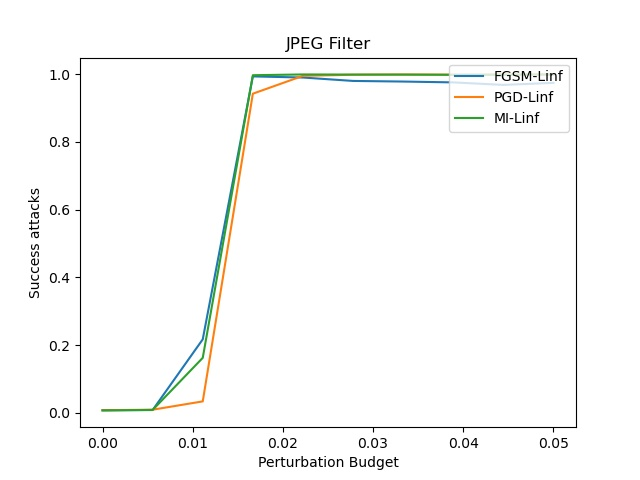
\includegraphics[width=0.49\linewidth]{images/exp3/untargeted/JPEG_Filter_succ.jpg}}
  \subcaptionbox{Bit squeezing\label{fig:subfig-d}}
    {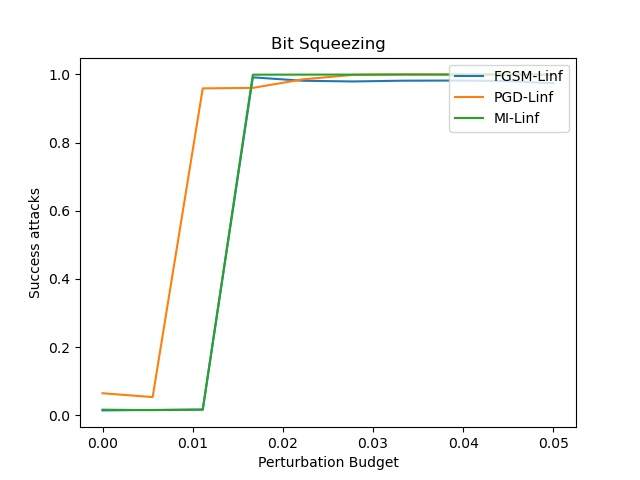
\includegraphics[width=0.49\linewidth]{images/exp3/untargeted/Bit_Squeezing_succ.jpg}}
  \subcaptionbox{No defense\label{fig:subfig-e}}
    {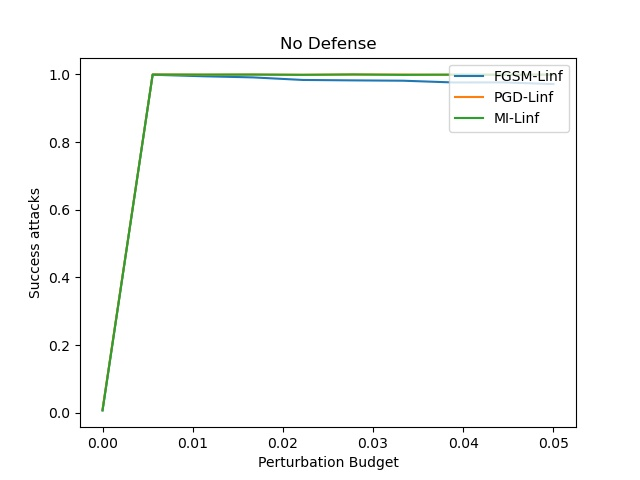
\includegraphics[width=0.49\linewidth]{images/exp3/untargeted/No_Defense_succ.jpg}}
  \caption{The {\it accuracy vs perturbation} curves of 5 DQN policies trained to play Pong and defended with 5 different defense methods (including no defense) under the \(l_\infty\) norm attacking with increased perturbations strength. Perturbations have been crafted in an untargeted way.}
  \label{figure:untargeted-suc}
\end{figure}

\subsection{Benchmark of targeted white-box attacks}
The charts relative to the {\it reward vs perturbation} and {\it accuracy vs perturbation} curves obtained under targeted settings are shown in figures \ref{figure:targeted-rew} and \ref{figure:targeted-suc} respectively. For each observation, the targeted action that has been selected is the action with the lowest probability. Hence, it is equal to adopt strategically-timed attack attacking all the possible observations. In terms of reward, FGSM is the attack that performs the worst against the two adversarial training-based defenses while the other two attacks obtain similar results. As for JPEG filter defense, the chart doesn't present any substantial difference among the curves of the evaluated attack methods. PGD is also the best attack to break bit squeezing defense. All curves begin to drop down for perturbations greater than 0.01 and the descent is steeper for JPEG filter and bit squeezing. As it was for the untargeted case, the value of the curves of the adversarial training-based defenses decreases more gradually and eventually reaches the bottom when \(\epsilon\) gets close to 0.03 or 0.04. The difference in terms of performance between adversarial training and the other two defenses is more significant when comparing their success rate curves. In fact, in the perturbations' strength interval taken into examination, targeted attacks against adversarial training protected policies work at most 20\% of the times while attacks against the other two defenses have a success rate of 100\% for \(\epsilon\) greater than 0.01. Under targeted settings, FGSM is the only attack whose accuracy never reaches 100\% against the undefended policy. It also shows an inferior performance against all the other defenses.

\begin{figure}
  \centering
  \subcaptionbox{FGSM adversarial training\label{fig:subfig-a}}
    {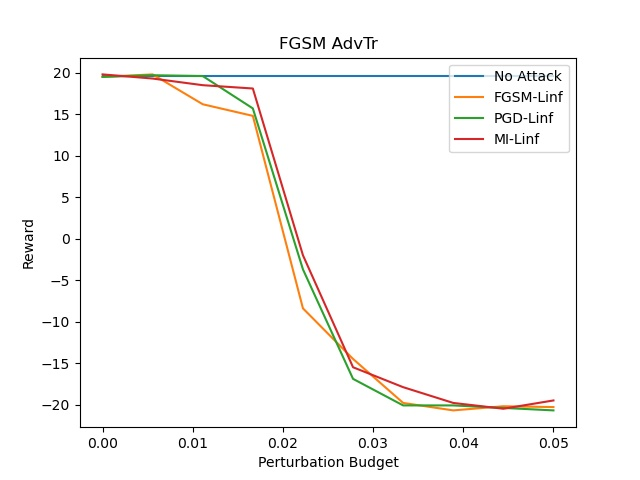
\includegraphics[width=0.49\linewidth]{images/exp3/targeted/FGSM_AdvTr.jpg}}
  \subcaptionbox{PPO adversarial training\label{fig:subfig-b}}
    {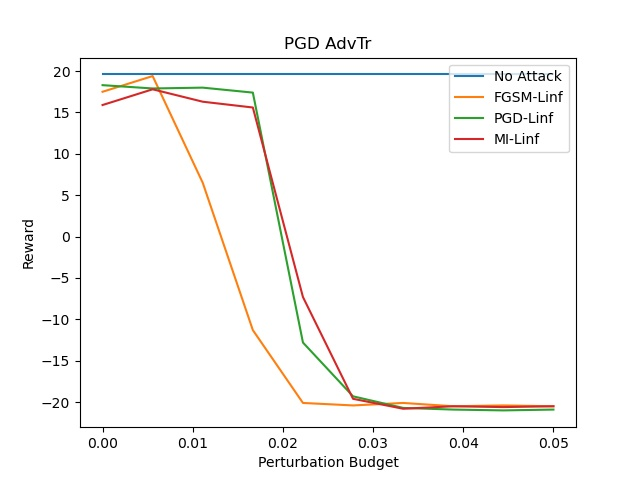
\includegraphics[width=0.49\linewidth]{images/exp3/targeted/PGD_AdvTr.jpg}}
  \subcaptionbox{JPEG filter\label{fig:subfig-c}}
    {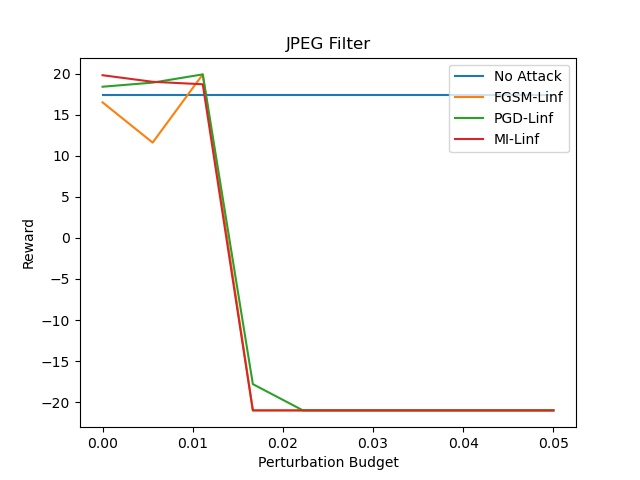
\includegraphics[width=0.49\linewidth]{images/exp3/targeted/JPEG_Filter.jpg}}
  \subcaptionbox{Bit squeezing\label{fig:subfig-d}}
    {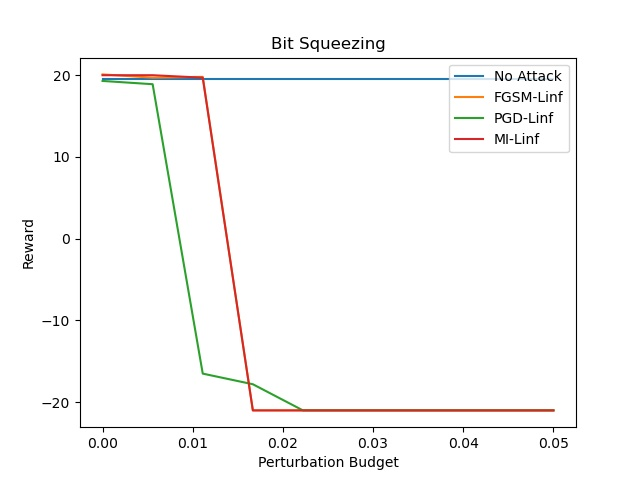
\includegraphics[width=0.49\linewidth]{images/exp3/targeted/Bit_Squeezing.jpg}}
  \subcaptionbox{No defense\label{fig:subfig-e}}
    {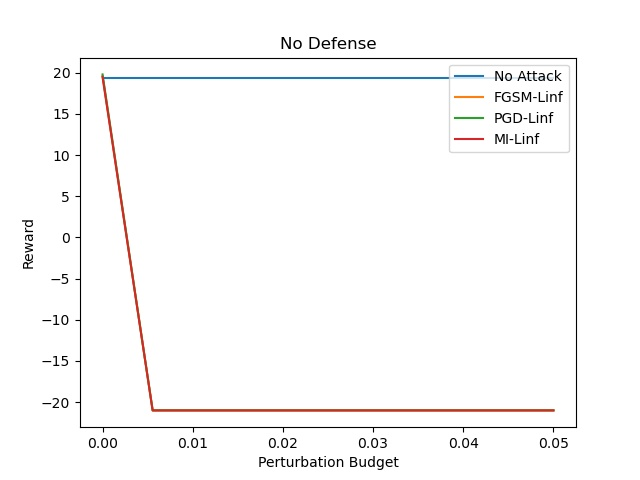
\includegraphics[width=0.49\linewidth]{images/exp3/targeted/No_Defense.jpg}}
  \caption{The {\it reward vs perturbation} curves of 5 DQN policies trained to play Pong and defended with 5 different defense methods (including no defense) under the \(l_\infty\) norm attacking with increased perturbations strength. Perturbations have been crafted in a targeted way.}
  \label{figure:targeted-rew}
\end{figure}

\begin{figure}
  \centering
  \subcaptionbox{FGSM adversarial training\label{fig:subfig-a}}
    {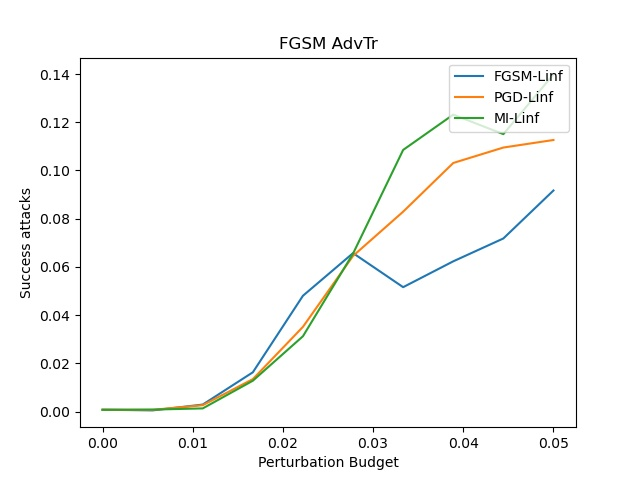
\includegraphics[width=0.49\linewidth]{images/exp3/targeted/FGSM_AdvTr_succ.jpg}}
  \subcaptionbox{PPO adversarial training\label{fig:subfig-b}}
    {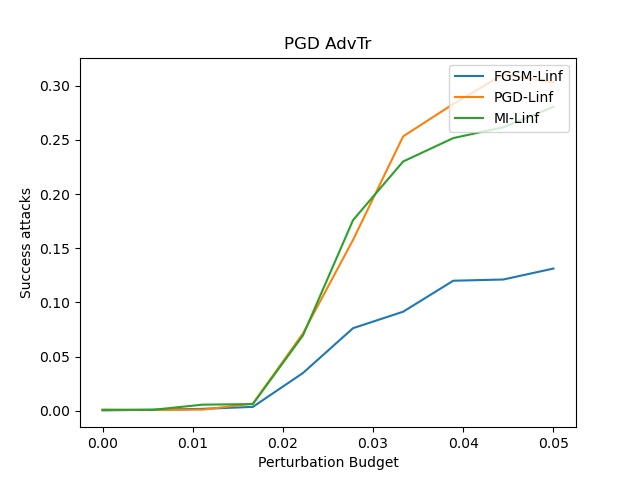
\includegraphics[width=0.49\linewidth]{images/exp3/targeted/PGD_AdvTr_succ.jpg}}
  \subcaptionbox{JPEG filter\label{fig:subfig-c}}
    {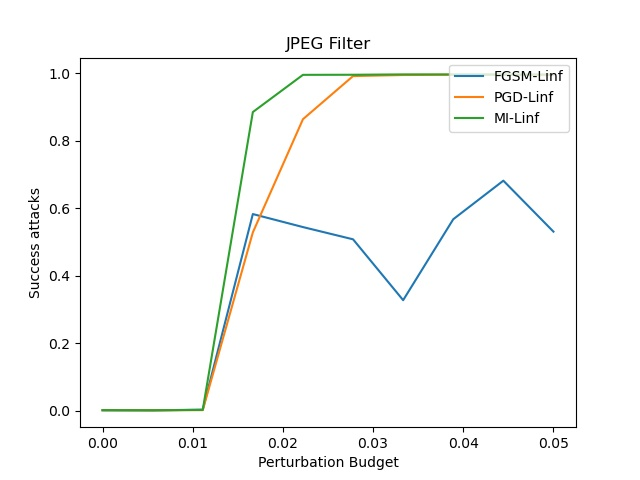
\includegraphics[width=0.49\linewidth]{images/exp3/targeted/JPEG_Filter_succ.jpg}}
  \subcaptionbox{Bit squeezing\label{fig:subfig-d}}
    {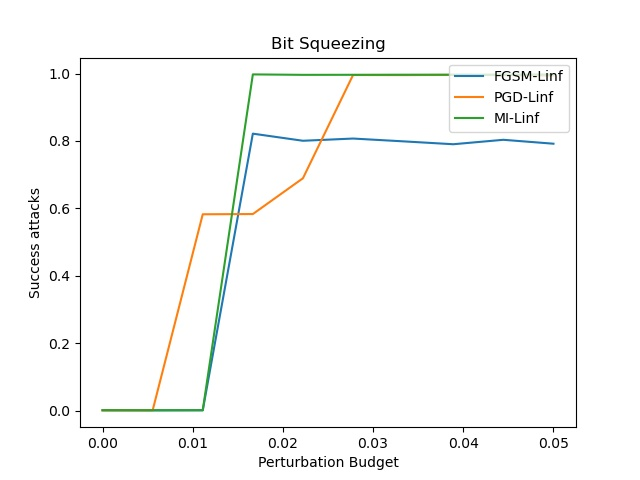
\includegraphics[width=0.49\linewidth]{images/exp3/targeted/Bit_Squeezing_succ.jpg}}
  \subcaptionbox{No defense\label{fig:subfig-e}}
    {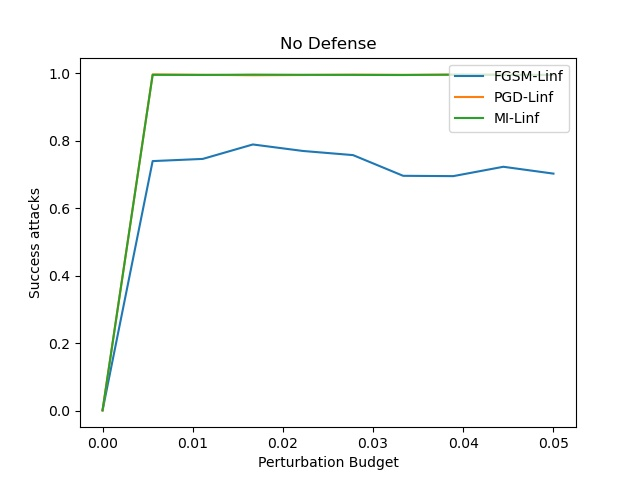
\includegraphics[width=0.49\linewidth]{images/exp3/targeted/No_Defense_succ.jpg}}
  \caption{The {\it accuracy vs perturbation} curves of 5 DQN policies trained to play Pong and defended with 5 different defense methods (including no defense) under the \(l_\infty\) norm attacking with increased perturbations strength. Perturbations have been crafted in a targeted way.}
  \label{figure:targeted-suc}
\end{figure}

\subsection{Findings}
This section shows the findings relative to the benchmark evaluated in this work. In particular, it makes some conclusions about the importance of this experiment, the differences between attacking under targeted and untargeted settings and it provides more insights about the evaluated defenses and their robustness.

\subsubsection{Importance of selecting the most appropriate image attack method}
Policy attacks based on image observations rely on image attacks to craft effective perturbations to fool their target agent. Hence, selecting the most effective image attack that performs better against a certain policy trained with a certain algorithm on a specific environment is a fundamental step to perform effective policy attacks.  In addition, different image attack methods might work better or worse against specific defense methods that protect the target policy. Thus, there are many variables that can condition the effectiveness of a policy attack. Also choosing the most appropriate threat model contributes to enhance the performance of the attacks and craft the most effective or imperceptible adversarial observations. For instance, in order to craft imperceptible adversarial examples, it is useful to know which minimal amount of \(\epsilon\) is enough to attack policy \(P\) defended with defense \(D\) on environment \(E\) or, given a fixed \(\epsilon\), it might be useful to find which attack shows the highest attack success rate or that reduces the agent's reward for the highest amount. Thus, reinforcement learning policies that take as input environment observations should have their robustness evaluated not only against policy attacks but also against image attack methods.

\subsubsection{Targeted and untargeted image attacks}
In this section, we are going to analyze the main differences that emerge when attacking under targeted and untargeted scenarios. Targeted attacks seem to be better at reducing the agent's reward but the probability that their attacks are executed correctly is significantly lower than their untargeted counterpart. However, they are still effective since most of the failed attacks, although they fail to fool the agent to select the selected action, they still corrupt the observations enough to fool the agent to take a random sub-optimal action. However, given a similar attack accuracy, targeted attacks can easily outperform untargeted attacks. For example, given the charts relative to the undefended policy, FGSM has 100\% accuracy under untargeted attack scenarios and a little more than 70\% accuracy under targeted settings. Nevertheless, its average reward for the untargeted case is a few points higher than its corresponding average reward obtained in the targeted scenario. This phenomenon is probably due to the fact that targeted attacks are more lethal and when they succeed they provoke greater damage to the victim policy. It is also worth noting that, in terms of accuracy, FGSM seems to suffer a loss in performance when attacking under targeted settings with respect to its targeted version. Overall, MI is the most effective attack under both settings. 

\subsubsection{Robustness of the evaluated defenses}
Among the evaluated policies, the most robust one seems to be the one defended with the two adversarial training-based methods, in fact, they offer great protection under both attack settings. PGD adversarial training is perhaps a little better than FGSM when comparing the success rate of malicious attacks. JPEG filter and feature squeezing reduce the quality of the input observations with the goal to smooth eventual malicious perturbations. The more the quality reduction, the more perturbations would be filtered out. However, an excessive quality reduction would also negatively affect the agent's performance. Hence, when those methods are used in practice, some attention should be put into finding the right tradeoff between performance and robustness. As we can see from table \ref{table:adv_def} adversarial training doesn't impact the agent's performance in a significant way. 

\subsubsection{Defenses applied during and after training}
One difference between adversarial training and the other two defenses that have been evaluated is that the first is applied during training while JPEG compression and feature squeezing have been applied only after training, that is during evaluation. Generally speaking, adversarial training should work better since the model learns to play following its policy in presence of perturbations. However, training the model for a longer time is costly and usually constrained to learn against perturbations crafted with just one type of attack method. Fortunately, adversarial training presents a sort of transferability, meaning that models defended with FGSM can also protect against PGD attacks and vice versa. This property is clearly shown in the charts in figure \ref{figure:untargeted-rew} and \ref{figure:targeted-rew}. JPEG compression and feature squeezing can still work against a large variety of attacks but the protection that they offer is often limited.

\subsubsection{Observations noise imperceptibility}
Given a fixed perturbations' strength \(\epsilon\), different image attacks can inject more or less perceptible noise to the target observations. Lower values of \(\epsilon\) usually lead to less visible perturbations, while higher values can make the target images too noisy and easily perceived by the human brain. Hence, to give an idea of the effect caused by the injection of noise to clear observations, we crafted four adversarial observations with FGSM and increasing values of \(\epsilon\) in the range [0.1, 0.01, 0.001, 0.0001] and compared them with clear observations. Then, we crafted other four adversarial observations with PGD and with the same values of \(\epsilon\). The noisy observations and the clear ones are shown in figure \ref{figure:pong-noise}. As we can immediately note in the figure, for similar \(\epsilon\) PGD crafts less perceptible adversarial observations than the one generated with FGSM. The injection of noise is visible in all the malicious observations generated with FGSM, while for adversarial examples generated with PGD, only the one crafted with \(\epsilon\) equal to 1 can be clearly detected. All perturbations have been crafted attacking a Pong-PPO model with \(l_\infty\) distance.

\begin{figure}
  \centering
  \subcaptionbox{\label{fig:subfig-a}}
    {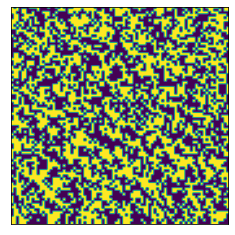
\includegraphics[width=0.19\linewidth]{images/noise/PongNoFrameskip-v4_gsm_ppo_eps_0.1.png}}
  \subcaptionbox{\label{fig:subfig-b}}
    {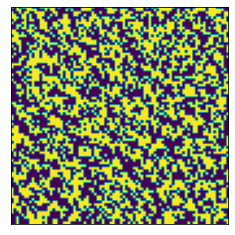
\includegraphics[width=0.19\linewidth]{images/noise/PongNoFrameskip-v4_gsm_ppo_eps_0.01.png}}
    \subcaptionbox{\label{fig:subfig-c}}
    {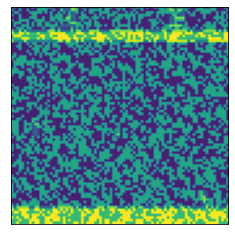
\includegraphics[width=0.19\linewidth]{images/noise/PongNoFrameskip-v4_gsm_ppo_eps_0.001.png}}
    \subcaptionbox{\label{fig:subfig-d}}
    {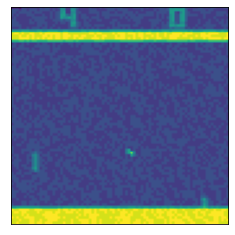
\includegraphics[width=0.19\linewidth]{images/noise/PongNoFrameskip-v4_gsm_ppo_eps_0.0001.png}}
    \subcaptionbox{\label{fig:subfig-e}}
    {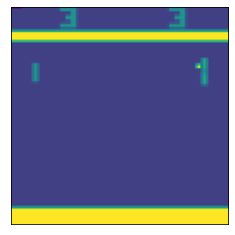
\includegraphics[width=0.19\linewidth]{images/noise/PongNoFrameskip-v4_gsm_ppo_eps_0.1_ori.png}}
    \subcaptionbox{\label{fig:subfig-f}}
    {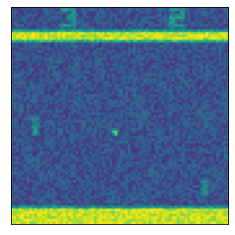
\includegraphics[width=0.19\linewidth]{images/noise/PongNoFrameskip-v4_pgda_ppo_eps_0.1.png}}
    \subcaptionbox{\label{fig:subfig-g}}
    {\includegraphics[width=0.19\linewidth]{images/noise/PongNoFrameskip-v4_pgda_ppo_eps_0.01.png}}
    \subcaptionbox{\label{fig:subfig-h}}
    {\includegraphics[width=0.19\linewidth]{images/noise/PongNoFrameskip-v4_pgda_ppo_eps_0.001.png}}
    \subcaptionbox{\label{fig:subfig-i}}
    {\includegraphics[width=0.19\linewidth]{images/noise/PongNoFrameskip-v4_pgda_ppo_eps_0.0001.png}}
    \subcaptionbox{\label{fig:subfig-j}}
    {\includegraphics[width=0.19\linewidth]{images/noise/PongNoFrameskip-v4_pgda_ppo_eps_0.1_ori.png}}
  \caption{{\bf First row}: Comparison of the effect of noise injections on Pong environment observations with different strength of perturbations. The most right one is a clear observation and from the right to the left have been injected noise with increasing perturbations \(\epsilon=[0.1, 0.01, 0.001, 0.0001]\). Perturbations have been crafted with FGSM attacking a policy trained with PPO. {\bf Second row}: Comparison of the effect of noise injections on Pong environment observations with different strength of perturbations. The most right one is a clear observation and from the right to the left have been injected noise with increasing perturbations \(\epsilon=[0.1, 0.01, 0.001, 0.0001]\). Perturbations have been crafted with PGD attacking a policy trained with PPO.}
  \label{figure:pong-noise}
\end{figure}

\section{Number of attacked policies}
One of the major difficulties encountered while carrying out this thesis work is the computation time taken to run all the experiments. For the first experiment have been evaluated 5 policy attacks against 3 reinforcement learning algorithms trained on 2 environments. Each policy has been attacked 4 times corresponding to the four curves shown on each chart: attacking without transferability, attacking a surrogate policy, and attacking two different surrogate algorithms. Each curve has been drawn out of 10 different attack frequencies corresponding to ten points along the \(x\)-axis. Uniform attack, since it is the fastest attack, has its corresponding curves containing 20 points. Moreover, each point has been computed as average of 10 runs. Thus, in total have been attacked at least \(5*3*2*4*10*10=12000\) policies. The second experiment instead evaluates 2 policy attacks against 3 reinforcement learning algorithms trained in a single environment. Similarly, each policy has been attacked 4 times corresponding to the four curves shown on each chart as in the previous experiment. Given that each curve is composed of 10 points averaged over 10 runs, in total have been attacked at least \( 2*3*1*4*10*10=2400\) policies. Finally in the third experiment have been evaluated 6 policies trained with DQN where 5 of them were defended with a defense mechanism and trained on the Pong environment. Each policy has been attacked with 3 different white-box attack methods and each curve is composed of 20 points taken over an average of 10 runs. The experiment has been conducted on both targeted and untargeted threat models. Hence, in total have been attacked \(6*3*2*20*10=7200\) policies. Hence, the whole work includes a total of 12000+2400+7200=21600 policy attacks. It took about two months using between 4 and 8 GeForce GTX TITAN X GPUs. In practice, more experiments have been conducted while tuning the attacks' hyper-parameters and verifying the correctness of all the implemented attacks.

\section{Implementation details}
In this section, we are going to discuss the details relative to the implementation of the evaluated reinforcement learning algorithms, the policy attacks, and the image attacks. The Github repository containing the code to obtain the results presented in this thesis is available at the following address: \url{https://github.com/davide97l/rl-policies-attacks-defenses}. It has been developed with Pytorch but relies on other frameworks, each specialized in a different task. The reinforcement learning algorithms have been taken from the framework \href{https://github.com/davide97l/rl-policies-attacks-defenses}{Tianshou} \cite{tianshou} developed by \href{http://ml.cs.tsinghua.edu.cn/}{TSAIL}. It consists of a reinforcement learning platform based on pure PyTorch and with support to parallelized environments. Image adversarial attacks have been taken from \href{https://github.com/BorealisAI/advertorch}{Advertorch} \cite{ding2019advertorch} developed by \href{https://www.borealisai.com/en/}{BorealisAI}. Advertorch is a Python toolbox for adversarial robustness research also based on PyTorch. Given that the model interface required by Advertorch is different from the one required by the model trained with Tianshou, it has been created an adapter class to adapt Tianshou models to Advertorch models. The two simple image defenses, namely JPEG conversion and feature squeezing have been implemented from scratch. Policy adversarial training has been developed from scratch and integrated into Tianshou. It expands the Tianshou classes implementing the training procedure of the normal policies to defend them with adversarial training. Policy attacks have also been implemented from scratch and made compatible with Tianshou. Their modularized code allows to easily develop new attacks by expanding a base class or any of the existing policies. Hence, the result of this work is also a framework to test the robustness of reinforcement learning trained policies. Finally, the Atari environments have been taken from the Gym library developed by \href{https://openai.com/}{OpenAI}. The same library also includes other well-studied environments made publicly available to the AI community.
\chapter{Conclusions}
\label{sec:conclusions}

\section{Summary}
In this work, we conducted three experiments to study the robustness of reinforcement learning policies and their defenses. In the first part, we focused on studying policy attacks transferability over policies and algorithms. We did it by computing the {\it reward vs attack frequency} curves of different policy attacks under a fixed threat model so to measure their effectiveness and their transferability against policies and algorithms. We repeated the experiment for a total of 3 algorithms, 5 policy attacks, and 2 environments. In the second experiment, we studied policy attacks transferability against defended policies. We did it by computing the {\it reward vs attack frequency} curves of different policy attacks under a fixed threat model so to measure their effectiveness and their transferability against defended policies and defended algorithms. We repeated the experiment for a total of 3 algorithms, 2 policy attacks, and 2 environments. The third and last experiment consisted of a benchmark to measure the robustness of defended policies against white-box image attacks methods. We compared the curves of victim policies’ average reward and the success rate of different white-box attack methods attacking input observations under a fixed threat model and over increasing values of perturbations’ strength. Victim policies have been protected with different defense methods.

\section{Future research directions}
The present experiment, even if it took a lot of work, can still be expanded to make it more complete. The algorithms that have been examined only include DQN, A2C, and PPO, but many other more or less novel algorithms could be added to this work. For instance, DQN has many more variants worth being tested such as C51-DQN \cite{bellemare2017distributional} and the more powerful Rainbow-DQN \cite{hessel2017rainbow}. Similarly, future work may also introduce new defenses to make the evaluated policies more robust. Many of them combine adversarial training with auxiliary loss functions to train policies with certified robustness \cite{wang2020adversarial} \cite{fischer2019online} \cite{zhang2020robust} \cite{oikarinen2020robust}. The main image attack used as a backbone by the policy attacks is FGSM and attacks relying on the two iterative methods, PGD and MI, have only been partially studied in the last experiment. However, this work could be extended by evaluating more diverse white-box attacks such as C\&W \cite{carlini2016evaluating} and Deepfool \cite{moosavidezfooli2016deepfool}. Instead of only focusing on black-box attacks, it could be interesting to know whether some black-box attacks could further boost the performance of the policy attacks. The only environments that have been explored in this work are simple Atari games with discrete actions. However, in some real scenarios, it is common to have to solve reinforcement learning tasks whose agent has to take continuous actions to interact with the environments. For example, most environments included in the categories MuJoco and Box2D have a continuous actions space which would cause the current implementations of DQN, A2C, and PPO to be useless. Hence, future work might also take into consideration to test the robustness of models specialized to deal with continuous actions environments such as SAC \cite{haarnoja2018soft}, TD3 \cite{fujimoto2018addressing} and DDPG \cite{lillicrap2019continuous}. Another possible scenario is when it is not possible to directly inject noise to the input observations but it is possible to generate adversarial observations by training a malicious agent to interact with the environment in a way such as to fool the victim agent. Under this particular scenario, new kinds of attacks and defenses are possible in order to test the robustness of the target policies.


% 其他部分
\backmatter

% 参考文献
% References
\bibliography{ref/refs}  % 参考文献使用 BibTeX 编译
% \printbibliography       % 参考文献使用 BibLaTeX 编译

% 附录
% Appendix
\appendix
%\input{data/appendix}
% % !TeX root = ../thuthesis-example.tex

% PLEASE IGNORE THIS PART! This is not applicable to Master students




\begin{survey}
\label{cha:survey}

\title{Title of the Survey}
\maketitle


\tableofcontents


本科生的外文资料调研阅读报告。


\section{Figures and Tables}

\subsection{Figures}

An example figure in appendix (Figure~\ref{fig:appendix-survey-figure}).

\begin{figure}
  \centering
  \includegraphics[width=0.6\linewidth]{example-image-a.pdf}
  \caption{Example figure in appendix}
  \label{fig:appendix-survey-figure}
\end{figure}


\subsection{Tables}

An example table in appendix (Table~\ref{tab:appendix-survey-table}).

\begin{table}
  \centering
  \caption{Example table in appendix}
  \begin{tabular}{ll}
    \toprule
    File name       & Description                                         \\
    \midrule
    thuthesis.dtx   & The source file including documentaion and comments \\
    thuthesis.cls   & The template file                                   \\
    thuthesis-*.bst & BibTeX styles                                       \\
    thuthesis-*.bbx & BibLaTeX styles for bibliographies                  \\
    thuthesis-*.cbx & BibLaTeX styles for citations                       \\
    \bottomrule
  \end{tabular}
  \label{tab:appendix-survey-table}
\end{table}


\section{Equations}

An example equation in appendix (Equation~\eqref{eq:appendix-survey-equation}).
\begin{equation}
  \frac{1}{2 \symup{\pi} \symup{i}} \int_\gamma f = \sum_{k=1}^m n(\gamma; a_k) \mathscr{R}(f; a_k)
  \label{eq:appendix-survey-equation}
\end{equation}


\section{Citations}

Example citations in appendix.
\cite{abrahams99tex}
\cite{salomon1995advanced}
\cite{abrahams99tex,salomon1995advanced}


\bibliographystyle{unsrtnat}
\bibliography{ref/appendix}

\end{survey}
       % 本科生:外文资料的调研阅读报告
% % !TeX root = ../thuthesis-example.tex

\begin{translation}
\label{cha:translation}

\title{书面翻译题目}
\maketitle

\tableofcontents


本科生的外文资料书面翻译。


\section{图表示例}

\subsection{图}

附录中的图片示例(图~\ref{fig:appendix-translation-figure})。

\begin{figure}
  \centering
  \includegraphics[width=0.6\linewidth]{example-image-a.pdf}
  \caption{附录中的图片示例}
  \label{fig:appendix-translation-figure}
\end{figure}


\subsection{表格}

附录中的表格示例(表~\ref{tab:appendix-translation-table})。

\begin{table}
  \centering
  \caption{附录中的表格示例}
  \begin{tabular}{ll}
    \toprule
    文件名          & 描述                         \\
    \midrule
    thuthesis.dtx   & 模板的源文件,包括文档和注释 \\
    thuthesis.cls   & 模板文件                     \\
    thuthesis-*.bst & BibTeX 参考文献表样式文件    \\
    thuthesis-*.bbx & BibLaTeX 参考文献表样式文件  \\
    thuthesis-*.cbx & BibLaTeX 引用样式文件        \\
    \bottomrule
  \end{tabular}
  \label{tab:appendix-translation-table}
\end{table}


\section{数学公式}

附录中的数学公式示例(公式~\eqref{eq:appendix-translation-equation})。
\begin{equation}
  \frac{1}{2 \symup{\pi} \symup{i}} \int_\gamma f = \sum_{k=1}^m n(\gamma; a_k) \mathscr{R}(f; a_k)
  \label{eq:appendix-translation-equation}
\end{equation}


\section{文献引用}

文献引用示例\cite{abrahams99tex}。


% 书面翻译的参考文献
\bibliographystyle{unsrtnat}
\bibliography{ref/appendix}

% 书面翻译对应的原文索引
\begin{translation-index}
  \nocite{salomon1995advanced}
  \bibliographystyle{unsrtnat}
  \bibliography{ref/appendix}
\end{translation-index}

\end{translation}
  % 本科生:外文资料的书面翻译

% 致谢
% Acknowledgements
% !TeX root = ../thuthesis-example.tex
% Acknowledgements
\begin{acknowledgements}
I want to thank my supervisor Zhu Jun for the support and guidance he gave me during the realization of this work. In particular, he provided me important feedback about the results that have been obtained and suggested me some interesting experiments to include in my work. I have also to thank Weng Jiayi, the main developer of Tianshou, for his useful discussions about the implementations of the reinforcement learning algorithms and the way to fine-tune their hyper-parameters specifically for the Atari games. Finally, I would like also to thank my family for the support they gave me during these two years at Tsinghua University and all the friends I met on campus for all the fantastic experiences lived together.
  
\end{acknowledgements}

% 声明
% Statement
%\statement
% 生成的声明页是否要插入页眉和页脚(默认 empty)
% 仅在需要进行电子签名时,才需要打开这一选项
% 插入的扫描声明页总是会生成页眉(研究生)和页脚,不受这一选项影响
\statement[page-style=plain]
% 将签字扫描后的声明文件 scan-statement.pdf 替换原始页面
% \statement[file=scan-statement.pdf]

% 个人简历、在学期间完成的相关学术成果
% Resume
% !TeX root = ../thuthesis-example.tex

\begin{resume}

  %\section*{Resume}
  % Please note the empty line to ensure the correct format for this section.
    Davide Liu was born on 27th August 1997 in Padova, Veneto, Italy. 
    
    He began his bachelor’s study in the Department of Computer Science, Padova University in September 2016, majoring in computer science, and got a Bachelor of Science degreeth in July 2019.
    
    He began his master’s study in the Department of Computer Science, Tsinghua University in September 2019, and is expected to get a Master of Science degree in Computer Science in July 2021.
    
    %She/He has started to pursue a doctor’s degree in Physics in the School/Department of XXX, Tsinghua University since September 2014. During this period, she/he has made academic achievements as follows.
    


  %\section*{Academic Achievements}

  % Please delete the following sections if they are not applicable.
  
  %\subsection*{\textbf{Monograph}}
  %\begin{achievements}
  %  \item Author. Title. Publishing Group. In standard referencing format
  %\end{achievements}
  %\subsection*{\textbf{Journal article}}
  % Please put your publications here
  %\begin{achievements}
  %  \item Yang Y, Ren T L, Zhang L T, et al. Miniature microphone with silicon-based ferroelectric thin films[J]. Integrated Ferroelectrics, 2003, 52:229-235.
  %  \item 杨轶, 张宁欣, 任天令, 等. 硅基铁电微声学器件中薄膜残余应力的研究[J]. 中国机械工程, 2005, 16(14):1289-1291.
   % \item 杨轶, 张宁欣, 任天令, 等. 集成铁电器件中的关键工艺研究[J]. 仪器仪表学报, 2003, 24(S4):192-193.
%    \item Yang Y, Ren T L, Zhu Y P, et al. PMUTs for handwriting recognition. In press[J]. (已被Integrated Ferroelectrics录用)
 % \end{achievements}


%  \subsection*{\textbf{Patent}}

%  \begin{achievements}
%    \item 任天令, 杨轶, 朱一平, 等. 硅基铁电微声学传感器畴极化区域控制和电极连接的方法: 中国, CN1602118A[P]. 2005-03-30.
%    \item Ren T L, Yang Y, Zhu Y P, et al. Piezoelectric micro acoustic sensor based on ferroelectric materials: USA, No.11/215, 102[P]. (American Patent number...)
%  \end{achievements}

\end{resume}


% 指导教师/指导小组学术评语
% Comments from the supervisor or reviewers
% !TeX root = ../thuthesis-example.tex

\chapter{COMMENTS FROM THESIS SUPERVISOR}

深度学习模型的对抗攻击与防御是当前研究的热点,是深度学习模型在应用过程中需要重点关注的问题。目前在图像识别等任务上,相关研究进展较多。但对于使用了深度神经网络的深度强化学习,这方面的研究相对较少。此外,对抗攻击与防御是矛与盾的关系,一方面的进展会促进另一方面的提升,因此,如何进行充分的评测是其中要解决的重要问题。 为此,该论文针对一些常见的深度强化学习算法的对抗鲁棒性进行评测,通过多个决策任务下的实验,展示它们在恶意策略攻击下的迁移性,同时,也对基于图像的对抗攻击进行了实验测试。 该论文的选题具有实际应用价值。作为一个实验验证的论文,相关实验在多个任务场景下开展,工作量充足,结论合理。论文写作符合规范。满足硕士论文的要求。


% 答辩委员会决议书
% Decision of the defense committee
% !TeX root = ../thuthesis-example.tex

\chapter{RESOLUTION OF THESIS DEFENSE COMMITTEE}

Adversarial attack and defense for deep learning is an important and timely topic that concerns the robustness of deep learning in real-world applications. Much work has been done on pattern recognition tasks, while the work on reinforcement learning is less yet increasing. Moreover, there is typically an arm race between attack and defense, thereby calling for comprehensive benchmarks. 

In this thesis, the author systematically studied adversarial robustness on deep reinforcement learning (DRL). It carried out a series of empirical studies of both attack and defense on various video games. Through the experimental results, the author shows the vulnerability of several representative DRL algorithms against attacks that design malicious policies, their transferability, and the ability of image-based attacks to craft effective adversarial observations, even in presence of defense mechanisms.

Through this thesis work, 刘大为 shows his solid knowledge on theoretical fundamentals, his professional knowledge, and his ability to conduct research independently. The thesis is well organized and written. During the oral defense, he presented his work clearly and answered questions correctly.
 
The defense committee voted unanimously in favor of 刘大为’s thesis, and recommended that the degree of Master of science be conferred on him. 


%%This thesis proposes...

%%The language of this section should be in concordance with the original document (either Chinese or English)

%%论文提出了……

%%论文取得的主要创新性成果包括:

%%1. ……

%%2. ……

%%3. ……

%%论文工作表明作者在×××××具有×××××知识,具有××××能力,论文××××,答辩××××。

%%答辩委员会表决,(×票/一致)同意通过论文答辩,并建议授予×××(姓名)×××(门类)学博士/硕士学位。


% 本科生的综合论文训练记录表(扫描版)
% \record{file=scan-record.pdf}

\end{document}
